\documentclass[11pt,a4paper]{article}
\usepackage[utf8]{inputenc}
\usepackage[T1]{fontenc}
\usepackage{amsmath,amssymb,amsfonts}
\usepackage{graphicx}
\usepackage{booktabs}
\usepackage{tabularx}
\usepackage{geometry}
\geometry{margin=1in}
\usepackage{cite}
\usepackage{url}
\usepackage{microtype}
\usepackage{hyperref}
\setlength{\emergencystretch}{3em}
\hypersetup{
    colorlinks=true,
    linkcolor=blue,
    citecolor=blue,
    urlcolor=blue
}

\title{\textbf{A Controlled Empirical Comparison of Classical and Quantum Kernel SVMs for Breast Cancer Classification}}

\author{
  \textbf{Sina Qasempour}\textsuperscript{1,*}\\[1ex]
  \textsuperscript{1}\textit{Independent Researcher, Iran}\\
  \textsuperscript{*}\textit{Corresponding author: qasempoursina@gmail.com}\\
  \textit{ORCID: \url{https://orcid.org/0009-0006-8853-6740}}
}

\date{September 2026}

\begin{document}

\maketitle

\begin{abstract}
Quantum kernels offer flexible similarity measures, but evidence for their practical value depends on controlled comparisons with tuned classical baselines. We compared linear and radial-basis-function support vector classifiers with ZZ-feature-map quantum support vector classifiers (QSVCs) on the Wisconsin Diagnostic Breast Cancer benchmark (569 samples and 30 features), treating malignant label 0 as positive. Across five predefined, overlapping stratified 80/20 partitions, preprocessing was fitted within each inner fold; QSVC repetition count, entanglement topology, and $C$ were jointly selected by five-fold inner cross-validation, frozen, refitted on the full outer-training set, and evaluated once on its outer test set. Mean malignant-class F1 was 0.934 for the inner-selected classical comparator versus 0.868 for QSVC after PCA to two dimensions, and 0.949 versus 0.872 after PCA to four dimensions; the classical comparator was higher on all five aligned splits. Exact Wilcoxon tests gave raw $p=0.0625$ and Holm-adjusted $p=0.1875$, so these dependent split-level results are descriptive and do not establish equivalence or population-level superiority. Exploratory ablation and fixed-hyperparameter sample-size analyses contextualized feature-map sensitivity but did not select the final architectures. Under the evaluated WDBC, PCA 2/4, 2Q/4Q, exact-statevector, and tested ZZ-feature-map conditions, no quantum advantage was observed.
\end{abstract}

\noindent\textbf{Keywords:} Quantum machine learning, Support Vector Classifier, Quantum kernel methods, ZZ feature map, Wisconsin Diagnostic Breast Cancer, Controlled empirical benchmark.

\bigskip
\hrule
\bigskip

\section{Introduction}

Kernel methods in machine learning operate by implicitly mapping input vectors from a classical data space into a higher-dimensional reproducing kernel Hilbert space (RKHS), where non-linear decision boundaries can be identified via convex quadratic programming~\cite{cortes1995support, scholkopf2002learning}. In recent years, quantum machine learning (QML) has extended this paradigm by encoding classical data vectors into quantum states via parameterized quantum circuits~\cite{havlicek2019supervised, schuld2019quantum}. By evaluating transition fidelities between prepared quantum states, a quantum processor evaluates a quantum kernel Gram matrix that may be classically intractable to compute, providing a theoretical foundation for potential quantum advantage in classification tasks~\cite{huang2021power, schuld2021supervised, liu2021rigorous}.

Despite this theoretical promise, empirical conclusions in QML are highly sensitive to experimental design, attainable problem scale, and the strength of classical comparators~\cite{bowles2024better, cerezo2022challenges, leither2026benchmarking}. Preprocessing before partitioning, evaluation on a single split, and comparison with untuned baselines can all produce misleading rankings~\cite{bowles2024better}. Circuit architecture and input scaling also determine the inductive bias of a quantum kernel~\cite{hubregtsen2021evaluation, shaydulin2022importance}. These concerns motivate comparisons that isolate preprocessing and model selection from held-out evaluation and that report simulation cost separately from predictive performance.

To address these methodological shortcomings, this study presents an end-to-end controlled empirical benchmark comparing classical SVMs (linear and radial-basis-function kernels) against QSVCs with parameterized ZZ feature maps. We examine two- and four-dimensional representations of WDBC using model-selection procedures fully nested within five fixed outer random splits. Complementary analyses investigate feature-map sensitivity, sample-size behavior, kernel geometry and alignment, and computational execution cost.

Under the evaluated conditions, no quantum advantage was observed for the tested dataset, preprocessing pipeline, qubit scale, and ZZ feature-map family. This scoped negative result does not address other datasets, embeddings, qubit counts, noisy devices, or physical QPU execution; its value lies in the controlled evidence it provides for this commonly used low-dimensional benchmark.

\subsection{Summary of Contributions}
This work makes five contributions:
\begin{enumerate}
    \item \textbf{Controlled model selection:} Fold-specific refitting of \texttt{StandardScaler}, PCA, quantum \texttt{MinMaxScaler}, and quantum Gram matrices during inner cross-validation, with deterministic joint inner selection of QSVC architecture and $C$ as well as classical model family and hyperparameters.
    \item \textbf{Paired multi-split evaluation:} Matched evaluation on five predefined seeds (\texttt{[42, 123, 456, 789, 2026]}), with exact Wilcoxon statistics, Holm correction, and explicitly exploratory split-level percentile bootstrap intervals.
    \item \textbf{Feature-map and sample-size analyses:} Ablation of repetitions and entanglement topology at two and four qubits, together with fixed-hyperparameter learning curves over $N_{\text{train}} \in \{50, 100, 200, 300, 455\}$.
    \item \textbf{Kernel-geometry analysis:} A $4^n$ operator-feature-space account of the fidelity kernel, with effective rank and centered kernel alignment used to relate geometry to predictive performance.
    \item \textbf{Reproducible negative benchmark:} Frozen results, per-fold selection records, predictions, figures, environment metadata, and validation scripts that make the scoped absence of quantum advantage auditable.
\end{enumerate}

\section{Research Questions}
To guide this controlled comparative investigation, we establish seven research questions:
\begin{itemize}
    \item \textbf{RQ1 (Accuracy):} Does the evaluated quantum kernel improve classification accuracy relative to tuned classical SVM baselines?
    \item \textbf{RQ2 (Predictive Metrics):} How do malignant-class F1 score and ROC-AUC compare between classical and quantum kernel machines?
    \item \textbf{RQ3 (Dimensionality Scaling):} How does QSVC behavior change when expanding from two to four PCA dimensions and corresponding qubits?
    \item \textbf{RQ4 (Computational Cost):} What measured CPU overhead does exact statevector kernel evaluation incur, and how should that measurement be distinguished from general scaling and QPU cost?
    \item \textbf{RQ5 (Quantum Kernel Geometry):} What similarity geometry, off-diagonal distribution, and spectral effective rank are induced by the quantum feature map?
    \item \textbf{RQ6 (Geometric Alignment):} How substantially does the quantum kernel geometry depart from the classical RBF similarity geometry as measured by Centered Kernel Alignment (CKA)?
    \item \textbf{RQ7 (Split Stability):} Are the observed empirical rankings stable across the five predefined, overlapping random train/test partitions?
\end{itemize}

\section{Related Work}
The literature contextualizing quantum kernel classifiers spans classical statistical learning theory, quantum circuit expressivity, kernel geometry, and empirical benchmarking rigor.

\subsection{Classical Kernel Methods and Inductive Biases}
Classical Support Vector Machines (SVMs) formulate pattern classification as the identification of a maximal-margin separating hyperplane in an inner-product space~\cite{cortes1995support, scholkopf2002learning}. When patterns are not linearly separable in their original representation, Mercer kernels $k(\mathbf{x}, \mathbf{x}') = \langle \phi(\mathbf{x}), \phi(\mathbf{x}') \rangle_{\mathcal{H}}$ implicitly project inputs into a reproducing kernel Hilbert space $\mathcal{H}$ without requiring explicit coordinate evaluation~\cite{cristianini2000introduction}. Linear and Gaussian radial-basis-function kernels provide established classical comparators, including in cancer-classification studies~\cite{guyon2002gene}. The experiments use scikit-learn's LibSVM-backed SVC implementation; its observed runtime depends on the data, solver behavior, and cache settings~\cite{chang2011libsvm, pedregosa2011scikit}.

\subsection{Quantum Feature Maps and Quantum Kernel Formulations}
Quantum kernel methods replace classical non-linear feature maps with quantum state preparation unitaries $U_\Phi(\mathbf{x})$ acting on an $n$-qubit reference state $|0^{\otimes n}\rangle$~\cite{havlicek2019supervised, schuld2019quantum}. This operation maps a classical vector $\mathbf{x} \in \mathbb{R}^d$ to a quantum pure state $|\psi(\mathbf{x})\rangle$ or density operator $\rho(\mathbf{x}) = |\psi(\mathbf{x})\rangle\langle\psi(\mathbf{x})|$. The corresponding kernel is evaluated as the quantum transition fidelity:
\begin{equation}
K(\mathbf{x}, \mathbf{x}') = |\langle \psi(\mathbf{x}) | \psi(\mathbf{x}') \rangle|^2 = \text{Tr}\left[\rho(\mathbf{x})\rho(\mathbf{x}')\right]
\end{equation}
Schuld demonstrated that supervised quantum classifiers trained with variational parameters are fundamentally linear models in quantum feature spaces, establishing formal equivalence between variational quantum classifiers (VQCs) and quantum kernel machines~\cite{schuld2021supervised}. The Second-Order Pauli-Z Expansion (\texttt{ZZFeatureMap}) proposed by Havl{\'i}{\v{c}}ek et al.~\cite{havlicek2019supervised} encodes features via single-qubit phase gates and entangles qubits using pairwise controlled-phase rotations. This architecture derives its theoretical motivation from instantaneous quantum polynomial (IQP) circuit families, for which classical sampling of the output distribution is conjectured to be intractable under standard complexity assumptions~\cite{bremner2016average, suzuki2020analysis}. However, Hubregtsen et al.~\cite{hubregtsen2021evaluation} observed that higher circuit entanglement does not correlate monotonically with improved classification accuracy, and alternative architectures such as data re-uploading~\cite{perezsalinas2020data} have been proposed to enhance expressivity.

\subsection{Quantum Kernel Generalization, Concentration, and Untrainability}
Quantum-kernel concentration is a recognized scalability concern related to, but distinct from, barren plateaus in variational optimization~\cite{mcclean2018barren, holmes2022connecting}. Thanasilp, Wang, Cerezo, and Holmes~\cite{thanasilp2024exponential} derived exponential concentration bounds under specified conditions involving embedding expressivity, entanglement, global measurements, or noise. For a fidelity kernel evaluated through a global overlap measurement, sufficiently small off-diagonal values may be indistinguishable with polynomially many shots, yielding an effectively uninformative estimated Gram matrix. These asymptotic results do not by themselves diagnose concentration in a two- or four-qubit exact-kernel experiment. K{\"u}bler, Buchholz, and Sch{\"o}lkopf~\cite{kubler2021inductive} analyzed the role of inductive bias and data alignment in quantum kernels, while Shaydulin and Wild~\cite{shaydulin2022importance} showed that input scaling functions as a kernel-bandwidth hyperparameter.

\subsection{Sample Complexity and Small-Data Regimes}
Generalization bounds show that some quantum models can generalize from limited training data when their effective complexity is controlled~\cite{caro2022generalization, banchi2021generalization}. In classical kernel regression, Canatar et al.~\cite{canatar2021spectral} related learning behavior to kernel spectra and task-model alignment. Such results characterize learnability under stated assumptions; they do not imply that a quantum kernel will be more sample-efficient than a tuned classical model on a given classical dataset. We therefore treat small-data performance as an empirical question rather than a presumed quantum advantage.

\subsection{Biomedical Benchmarking on Oncological Data}
Biomedical QML studies span materially different tasks. Wang~\cite{wang2024novel} combined a quantum SVM with multi-objective feature selection on a breast-cancer dataset, whereas Azevedo, Silva, and Dutra~\cite{azevedo2022quantum} studied hybrid quantum transfer learning on full-field mammograms rather than WDBC. Leither, Lubinski, Kubal, and Johri~\cite{leither2026benchmarking} reported broad comparisons across tabular, omics, and spatial oncology tasks and found no evidence of quantum advantage in the evaluated settings. These works are not directly performance-comparable with the present fixed WDBC protocol because their inputs, model families, selection procedures, and validation designs differ.

\subsection{Empirical Rigor and Quantum Advantage Claims}
Establishing genuine quantum advantage in machine learning requires navigating stringent theoretical and empirical hurdles~\cite{cerezo2022challenges, preskill2018quantum}. Aaronson~\cite{aaronson2015read} emphasized input/output caveats in claims of quantum speedup, and Tang~\cite{tang2019quantum} showed how comparable randomized-access assumptions can enable classical ``dequantization.'' In a benchmark of 12 quantum models across six tasks and 160 derived datasets, Bowles, Ahmed, and Schuld~\cite{bowles2024better} found that out-of-the-box classical methods generally performed better and emphasized the importance of experimental design and tuned baselines. Rigorous empirical benchmarking therefore requires identical partitions, fold-local preprocessing, and transparent selection rules.

\section{Dataset and Problem Formulation}
The empirical evaluation is conducted on the \textbf{Wisconsin Diagnostic Breast Cancer (WDBC)} dataset, originally compiled by Street, Wolberg, and Mangasarian~\cite{street1993nuclear} and distributed through scikit-learn~\cite{pedregosa2011scikit}.
\begin{itemize}
    \item \textbf{Sample Size:} $N = 569$ patient observations.
    \item \textbf{Feature Space:} 30 continuous real-valued features computed from digitized images of fine needle aspirates (FNA) of breast masses, describing characteristics of cell nuclei (e.g., radius, texture, perimeter, area, smoothness, compactness, concavity, concave points, symmetry, and fractal dimension across mean, standard error, and ``worst'' measurements).
    \item \textbf{Target Classes:} Binary classification:
    \begin{itemize}
        \item \textbf{Malignant:} 212 samples (37.26\%).
        \item \textbf{Benign:} 357 samples (62.74\%).
    \end{itemize}
    \item \textbf{Positive Class Designation:} \textbf{Malignant (Class 0)} is treated as the predefined positive class (\texttt{pos\_label=0}) across all precision, recall, F1, and ROC-AUC evaluations. Decision scores are oriented consistently to that label.
    \item \textbf{Methodological Scope Disclaimer:} This investigation is strictly designed as a methodological machine-learning benchmark evaluating kernel representations. It does \textbf{not} constitute a clinical validation study, and the resulting models are not intended for medical diagnostic decision-making.
\end{itemize}

\section{Experimental Protocol and Leakage Prevention}
The experimental architecture uses five predefined outer splits with nested inner cross-validation: \texttt{SEEDS = [42, 123, 456, 789, 2026]}~\cite{bowles2024better}.

\subsection{Partitioning Protocol}
\begin{enumerate}
    \item \textbf{Outer Split:} An 80/20 stratified partition divides the 569 samples into 455 training observations and 114 test observations. Outer test partitions remain completely quarantined during all preprocessing fitting and hyperparameter selection.
    \item \textbf{Inner Cross-Validation:} Within each outer training set ($N=455$), a 5-fold stratified cross-validation is performed (364 training, 91 validation per fold).
    \item \textbf{Fold-local preprocessing:} \texttt{StandardScaler}, \texttt{PCA}, and quantum \texttt{MinMaxScaler} are fitted exclusively on the training portion of the respective partition. They are applied to validation and test partitions strictly via \texttt{transform()}. During inner tuning, transformers and quantum Gram matrices are independently recomputed inside each fold.
\end{enumerate}

For the authoritative final comparison, the outer test data are not used in preprocessing, architecture selection, or hyperparameter selection. The same five outer partitions were also examined during earlier exploratory development and are reused by the descriptive ablation and sample-size analyses. The corrected final algorithm is therefore outer-test-isolated, but the study remains a post hoc analysis rather than independent confirmatory validation.

\subsection{Dimensionality Reduction}
Due to qubit scalability constraints in current quantum simulators and NISQ devices~\cite{preskill2018quantum}, the 30 standardized features are compressed using Principal Component Analysis (PCA):
\begin{itemize}
    \item \textbf{PCA 2:} 2 principal components capturing $63.5\% \pm 0.6\%$ of cumulative feature variance.
    \item \textbf{PCA 4:} 4 principal components capturing $79.4\% \pm 0.4\%$ of cumulative feature variance.
\end{itemize}

\section{Classical Support Vector Machine Baselines}
Classical benchmarks utilize the standard LibSVM implementation via scikit-learn~\cite{pedregosa2011scikit, chang2011libsvm}:
\begin{enumerate}
    \item \textbf{Linear SVM (\texttt{SVC(kernel='linear')}):} Linear decision hyperplane optimized over regularization parameter $C \in \{0.01, 0.1, 1.0, 10.0, 100.0\}$~\cite{cortes1995support}.
    \item \textbf{Radial Basis Function (RBF) SVM (\texttt{SVC(kernel='rbf')}):} Non-linear Gaussian kernel $K(\mathbf{x}, \mathbf{x}') = \exp(-\gamma \|\mathbf{x} - \mathbf{x}'\|^2)$ optimized over $C \in \{0.01, 0.1, 1.0, 10.0, 100.0\}$ and $\gamma \in \{\text{'scale'}, \text{'auto'}, 0.01, 0.1, 1.0\}$~\cite{scholkopf2002learning, guyon2002gene}.
    \item \textbf{Inner-Selected Classical Comparator:} To prevent selective reporting bias, the classical model family (Linear vs.\ RBF) and hyperparameter configuration achieving the highest mean inner-CV malignant F1 score is designated as the canonical classical comparator for that outer split~\cite{bowles2024better}. Ties are resolved deterministically by favoring smaller $C$, followed by Linear over RBF.
\end{enumerate}

Accuracy summarizes overall classification. Precision, recall, and F1 use malignant label 0 as the positive class. ROC-AUC is computed from negated decision scores so that larger scores indicate malignancy. Means and sample standard deviations summarize the five outer splits; only malignant-class F1 belongs to the predefined inferential family.

\section{Quantum Kernel Support Vector Classifier (QSVC)}

\subsection{Quantum Feature Map Formulation}
The quantum classifier maps classical feature vectors $\mathbf{x} \in [0, \pi]^n$ into an $n$-qubit quantum state space using the Second-Order Pauli-Z Expansion (\texttt{zz\_feature\_map}) implemented in Qiskit~\cite{qiskit2026, suzuki2020analysis}:
\begin{equation}
\mathcal{U}_{\Phi}(\mathbf{x}) = \prod_{d=1}^{\text{reps}} \left( \prod_{i < j} U_{\Phi_{i,j}}(\mathbf{x}) \prod_{k=1}^n U_{\Phi_k}(\mathbf{x}) H^{\otimes n} \right)
\end{equation}
where $H^{\otimes n}$ denotes a layer of Hadamard gates initializing an equal superposition, $U_{\Phi_k}(\mathbf{x}) = \exp(-i \Phi_k(\mathbf{x}) Z_k / 2)$ encodes individual features via single-qubit phase rotations with $\Phi_k(\mathbf{x}) = 2 x_k$, and $U_{\Phi_{i,j}}(\mathbf{x}) = \exp(-i \Phi_{i,j}(\mathbf{x}) Z_i Z_j / 2)$ encodes pairwise non-linear interactions via two-qubit controlled-phase gates with:
\begin{equation}
\Phi_{i,j}(\mathbf{x}) = 2(\pi - x_i)(\pi - x_j)
\end{equation}
As demonstrated by Shaydulin and Wild~\cite{shaydulin2022importance}, mapping input components to $[0, \pi]$ sets an effective bandwidth scale for the statevector encoding.

\subsection{Fidelity Kernel and Operator Feature Space}
The similarity between two classical samples $\mathbf{x}_i$ and $\mathbf{x}_j$ is defined by the quantum state transition fidelity~\cite{havlicek2019supervised, schuld2019quantum}:
\begin{equation}
K(\mathbf{x}_i, \mathbf{x}_j) = |\langle \psi(\mathbf{x}_i) | \psi(\mathbf{x}_j) \rangle|^2 = \text{Tr}\left[ \rho(\mathbf{x}_i) \rho(\mathbf{x}_j) \right]
\end{equation}
where $\rho(\mathbf{x}) = |\psi(\mathbf{x})\rangle\langle\psi(\mathbf{x})|$ is the pure state density operator.

\noindent\textbf{Operator Feature Space Formulation:} As demonstrated by Schuld~\cite{schuld2021supervised}, although the underlying quantum statevectors $|\psi(\mathbf{x})\rangle$ reside in an $n$-qubit complex Hilbert state space $\mathcal{H} = \mathbb{C}^{2^n}$ of dimension $2^n$, the fidelity kernel mathematically evaluates the Hilbert-Schmidt inner product of density operators in the linear operator space $\mathcal{B}(\mathcal{H}) \cong \mathcal{H} \otimes \mathcal{H}^*$. The linear dimension of this operator feature space scales as:
\begin{equation}
\dim \mathcal{B}(\mathcal{H}) = (2^n)^2 = 4^n
\end{equation}
(or $4^n - 1$ for the subspace of traceless Hermitian operators). Consequently, the maximum algebraic rank of the fidelity Gram matrix is $\min(N, 4^n)$---scaling up to $16$ for $n=2$ qubits ($4^2 = 16$) and up to $256$ for $n=4$ qubits ($4^4 = 256$)---rather than being bounded by the statevector dimension $2^n$.

\subsection{Statevector Simulation Engine}
Kernel matrices are evaluated exactly for the specified noiseless feature map via statevector linear algebra on classical CPUs:
\begin{equation}
K_{ij} = \left|\langle \psi(\mathbf{x}_i) \mid \psi(\mathbf{x}_j) \rangle\right|^2
\end{equation}
Equivalently, if $\mathbf{\Psi} \in \mathbb{C}^{N \times 2^n}$ is the matrix whose rows are statevectors, each entry of $\mathbf{\Psi}\mathbf{\Psi}^{\dagger}$ is converted to its element-wise squared modulus. Gram matrix diagonals are explicitly enforced to $K_{i,i} = 1.0$, and numerical symmetry and positive semi-definiteness ($\text{eigvals} \ge -10^{-10}$) are verified.

\noindent\textbf{Simulation vs.\ Hardware Distinction:} Exact statevector simulation evaluates mathematical inner products directly without shot noise, gate infidelities, or decoherence~\cite{peters2021machine}. It provides an ideal representation of the feature-map geometry but does \textbf{not} represent physical quantum processor (QPU) execution latencies.

\subsection{Authoritative Nested QSVC Selection}
Within each outer-training set, five-fold inner cross-validation jointly searches $\text{reps}\in\{1,2,3\}$, entanglement topology, and $C\in\{0.01,0.1,1,10,100\}$. For 2Q, linear is the single canonical topology because linear and full are algebraically equivalent when only the pair $(0,1)$ exists; for 4Q, both linear and full are searched. Mean inner-fold malignant-class F1 determines the configuration. Deterministic ties are resolved by lower repetition count, linear before full, and smaller $C$. The selected configuration is frozen, all preprocessing is refitted on the complete outer-training set, and the outer test set is evaluated once.

All ten representation/seed selections chose $\text{reps}=1$. The 2Q selections used $C=100,100,1,10,10$ for seeds 42, 123, 456, 789, and 2026, respectively; all five 4Q selections chose full entanglement and $C=1$. Per-seed records and selection frequencies are reported in the Supplementary Material. These decisions come from the corrected nested search, not from the exploratory ablation in Section~\ref{sec:ablation}.

\section{Exploratory Quantum Feature-Map Ablation Study}\label{sec:ablation}
To describe the sensitivity of quantum kernel representations to circuit depth and entanglement topology, we conducted an exploratory 60-run ablation across circuit repetitions ($\text{reps} \in \{1, 2, 3\}$), entanglement topologies (\texttt{'linear'} vs.\ \texttt{'full'}), and qubit dimensions ($q \in \{2, 4\}$) across all five outer splits~\cite{hubregtsen2021evaluation}. Because it reports outer-test behavior, this phase is descriptive and is not the source of the final QSVC architecture selections.

\begin{figure}[htbp]
\centering
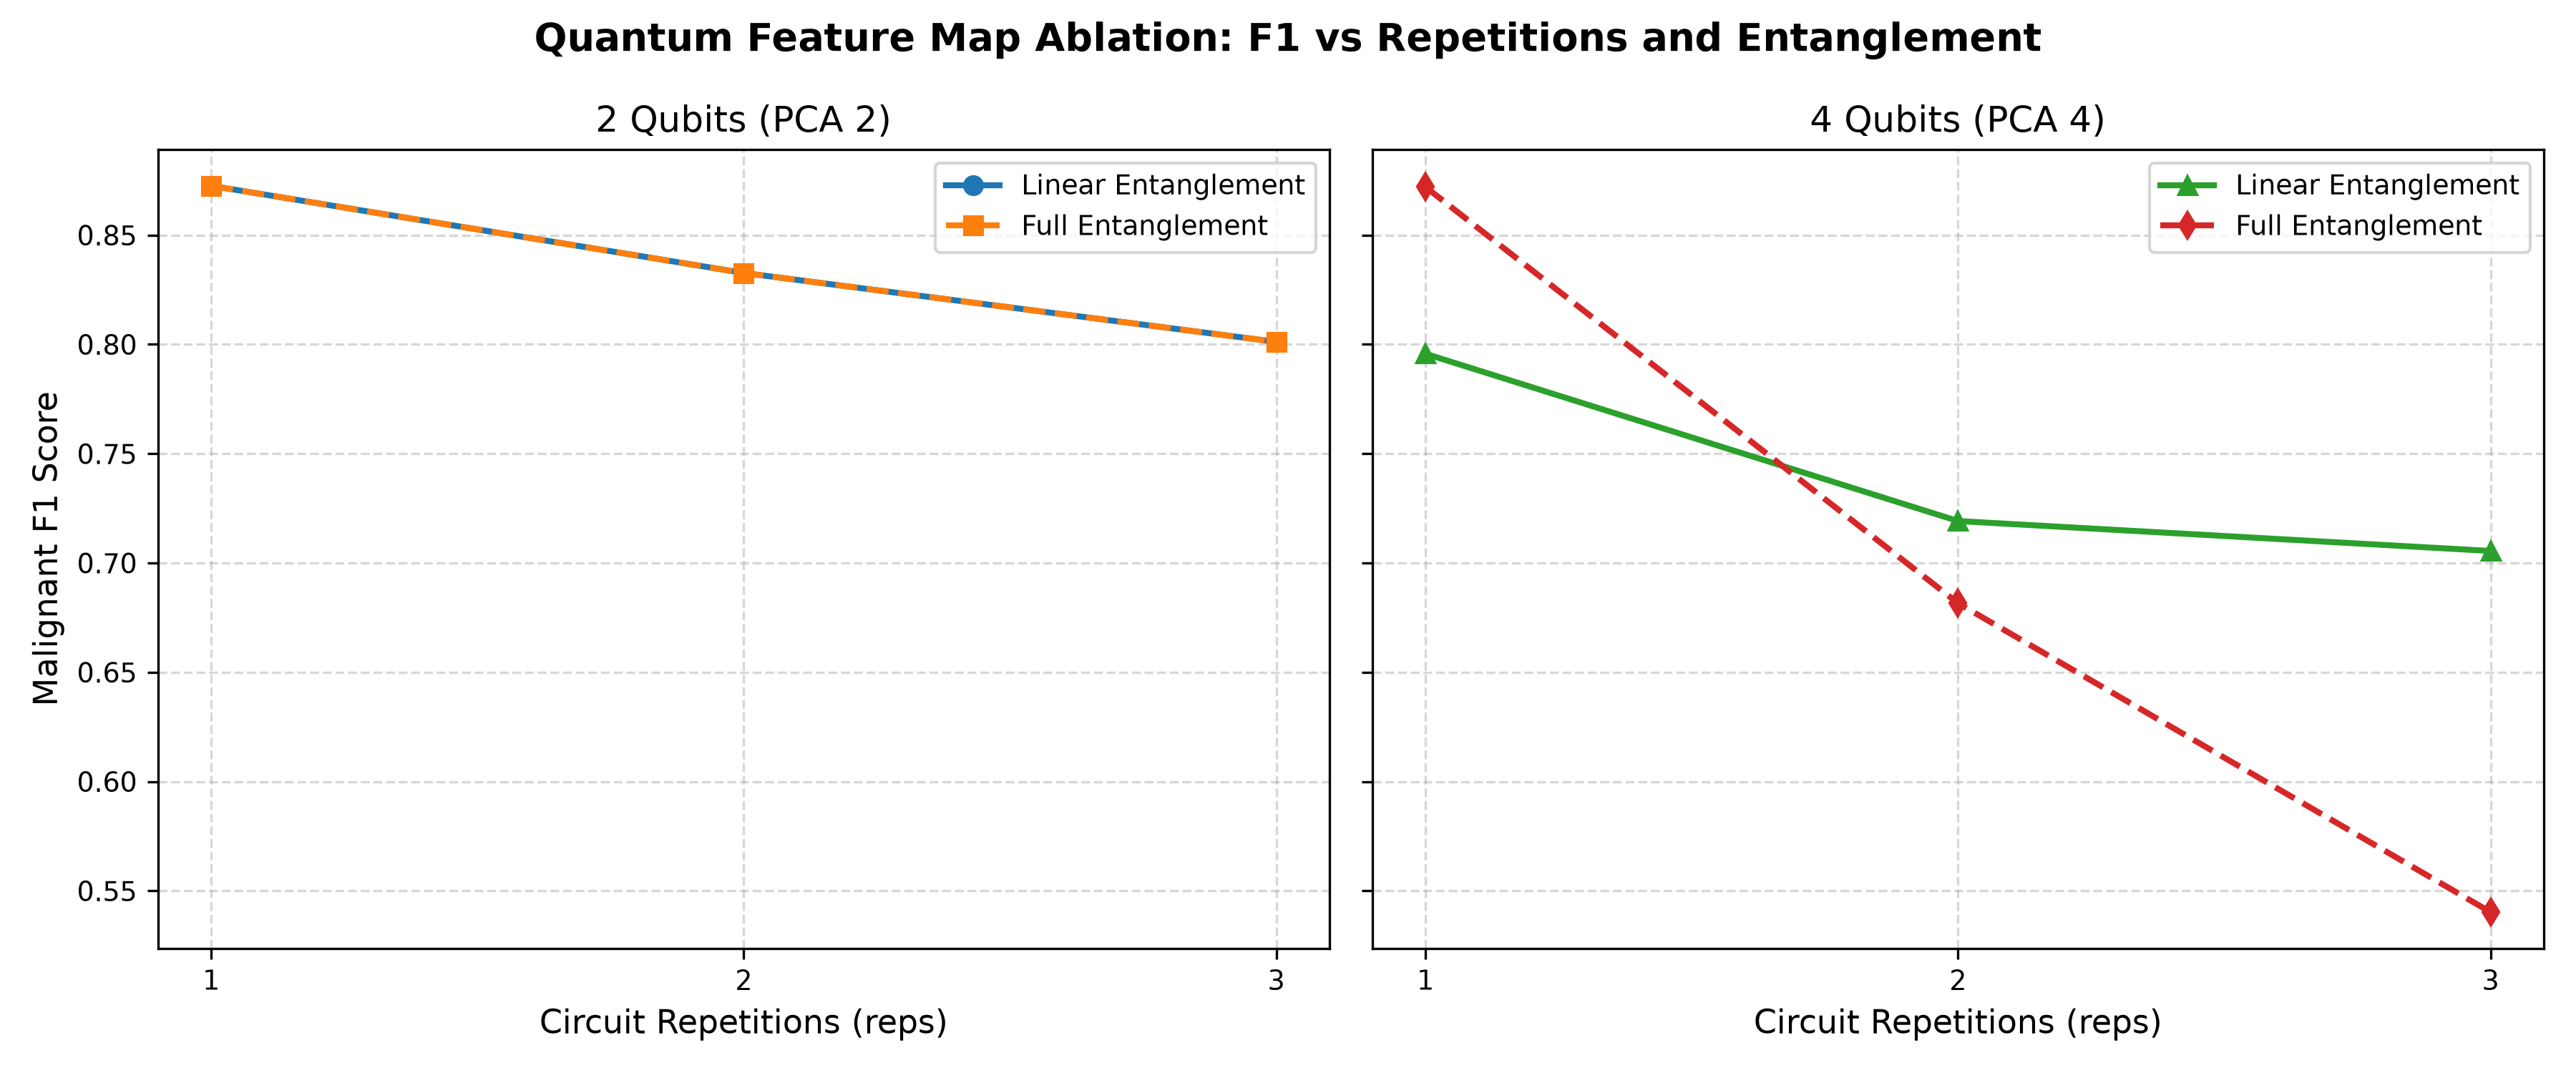
\includegraphics[width=0.95\textwidth]{figures/final_feature_map_ablation.png}
\caption{\textbf{Quantum Feature-Map Ablation Dynamics.} Outer-test malignant F1 across circuit repetitions ($\text{reps} \in \{1, 2, 3\}$), entanglement topology (\texttt{linear} vs.\ \texttt{full}), and 2- or 4-qubit representations. These descriptive results show an association between the tested architectures and performance; they do not isolate a single causal mechanism.}
\label{fig:ablation}
\end{figure}

\begin{table}[htbp]
\centering
\caption{Quantum Feature-Map Ablation across 5 Outer Splits ($n=60$ Quantum Runs, Mean $\pm$ SD).}
\label{tab:ablation}
\vspace{2mm}
\resizebox{\textwidth}{!}{%
\begin{tabular}{ccccccccc}
\toprule
Qubits ($q$) & Reps & Entanglement & Outer Malignant F1 & Outer ROC-AUC & Outer Accuracy & Off-Diag Mean & Off-Diag Std & Effective Rank \\
\midrule
2 & 1 & Linear & $0.8726 \pm 0.0376$ & $0.9697 \pm 0.0141$ & $0.9123 \pm 0.0224$ & $0.3244 \pm 0.0071$ & $0.2908 \pm 0.0039$ & $7.35 \pm 0.21$ \\
2 & 1 & Full & $0.8726 \pm 0.0376$ & $0.9697 \pm 0.0141$ & $0.9123 \pm 0.0224$ & $0.3244 \pm 0.0071$ & $0.2908 \pm 0.0039$ & $7.35 \pm 0.21$ \\
2 & 2 & Linear & $0.8327 \pm 0.0283$ & $0.9414 \pm 0.0240$ & $0.8842 \pm 0.0169$ & $0.4311 \pm 0.0302$ & $0.2795 \pm 0.0033$ & $6.33 \pm 0.50$ \\
2 & 2 & Full & $0.8327 \pm 0.0283$ & $0.9414 \pm 0.0240$ & $0.8842 \pm 0.0169$ & $0.4311 \pm 0.0302$ & $0.2795 \pm 0.0033$ & $6.33 \pm 0.50$ \\
2 & 3 & Linear & $0.8012 \pm 0.0352$ & $0.9204 \pm 0.0250$ & $0.8596 \pm 0.0215$ & $0.4818 \pm 0.0249$ & $0.2677 \pm 0.0015$ & $5.90 \pm 0.40$ \\
2 & 3 & Full & $0.8012 \pm 0.0352$ & $0.9204 \pm 0.0250$ & $0.8596 \pm 0.0215$ & $0.4818 \pm 0.0249$ & $0.2677 \pm 0.0015$ & $5.90 \pm 0.40$ \\
\midrule
4 & 1 & Linear & $0.7957 \pm 0.0688$ & $0.9263 \pm 0.0303$ & $0.8596 \pm 0.0345$ & $0.0818 \pm 0.0041$ & $0.1306 \pm 0.0072$ & $70.29 \pm 4.94$ \\
\textbf{4} & \textbf{1} & \textbf{Full} & $\mathbf{0.8721 \pm 0.0556}$ & $\mathbf{0.9581 \pm 0.0227}$ & $\mathbf{0.9053 \pm 0.0423}$ & $\mathbf{0.0961 \pm 0.0032}$ & $\mathbf{0.1015 \pm 0.0046}$ & $\mathbf{96.49 \pm 5.41}$ \\
4 & 2 & Linear & $0.7192 \pm 0.0859$ & $0.8935 \pm 0.0442$ & $0.8140 \pm 0.0423$ & $0.0829 \pm 0.0035$ & $0.1057 \pm 0.0046$ & $95.80 \pm 5.39$ \\
4 & 2 & Full & $0.6816 \pm 0.0590$ & $0.8546 \pm 0.0482$ & $0.7789 \pm 0.0364$ & $0.0811 \pm 0.0015$ & $0.0845 \pm 0.0019$ & $123.66 \pm 2.65$ \\
4 & 3 & Linear & $0.7055 \pm 0.0493$ & $0.8700 \pm 0.0311$ & $0.7965 \pm 0.0413$ & $0.0977 \pm 0.0025$ & $0.1080 \pm 0.0031$ & $93.63 \pm 4.01$ \\
4 & 3 & Full & $0.5403 \pm 0.0523$ & $0.7872 \pm 0.0340$ & $0.7228 \pm 0.0295$ & $0.0778 \pm 0.0018$ & $0.0770 \pm 0.0017$ & $137.43 \pm 2.83$ \\
\bottomrule
\end{tabular}%
}
\end{table}

\subsection{Key Empirical Findings}
\begin{enumerate}
    \item \textbf{Two-Qubit Regimes:} In 2Q, linear and full entanglement are algebraically identical because only a single qubit pair $(0,1)$ exists. As circuit depth increases, outer-test malignant F1 degrades monotonically ($\text{reps}=1$: $0.8726$; $\text{reps}=2$: $0.8327$; $\text{reps}=3$: $0.8012$).
    \item \textbf{Four-Qubit Regimes:} In 4Q, circuit depth exhibits an acute interaction with entanglement. Full entanglement with $\text{reps}=1$ achieves the strongest performance ($0.8721 \pm 0.0556$), whereas deeper configurations collapse severely ($\text{reps}=3$, Full: $0.5403 \pm 0.0523$).
\end{enumerate}

\subsection{Conservative Methodological Interpretation}
Within the tested 4Q full-entanglement configurations, greater repetition count was associated with lower F1 and broader effective-rank diagnostics. The design does not isolate depth from all other representation effects, and two qubit counts cannot establish an asymptotic concentration law. We therefore describe the pattern as concentration-like rather than as proof that depth caused a model collapse~\cite{thanasilp2024exponential, holmes2022connecting}.

\section{Sample-Size Scaling Dynamics}
We evaluated model performance across nested training subsets $N_{\text{train}} \in \{50, 100, 200, 300, 455\}$ with preprocessing refit on each subset and evaluation on the fixed outer test sets ($N_{\text{test}}=114$). These learning curves use fixed classifier settings---$C=1$ for every SVC, \texttt{gamma='scale'} for RBF, and \texttt{reps}=1 with full entanglement for QSVC---rather than the authoritative nested-selected settings. They therefore address sample-size behavior under a controlled fixed-hyperparameter protocol and should not be read as the tuned final comparison.

\begin{figure}[htbp]
\centering
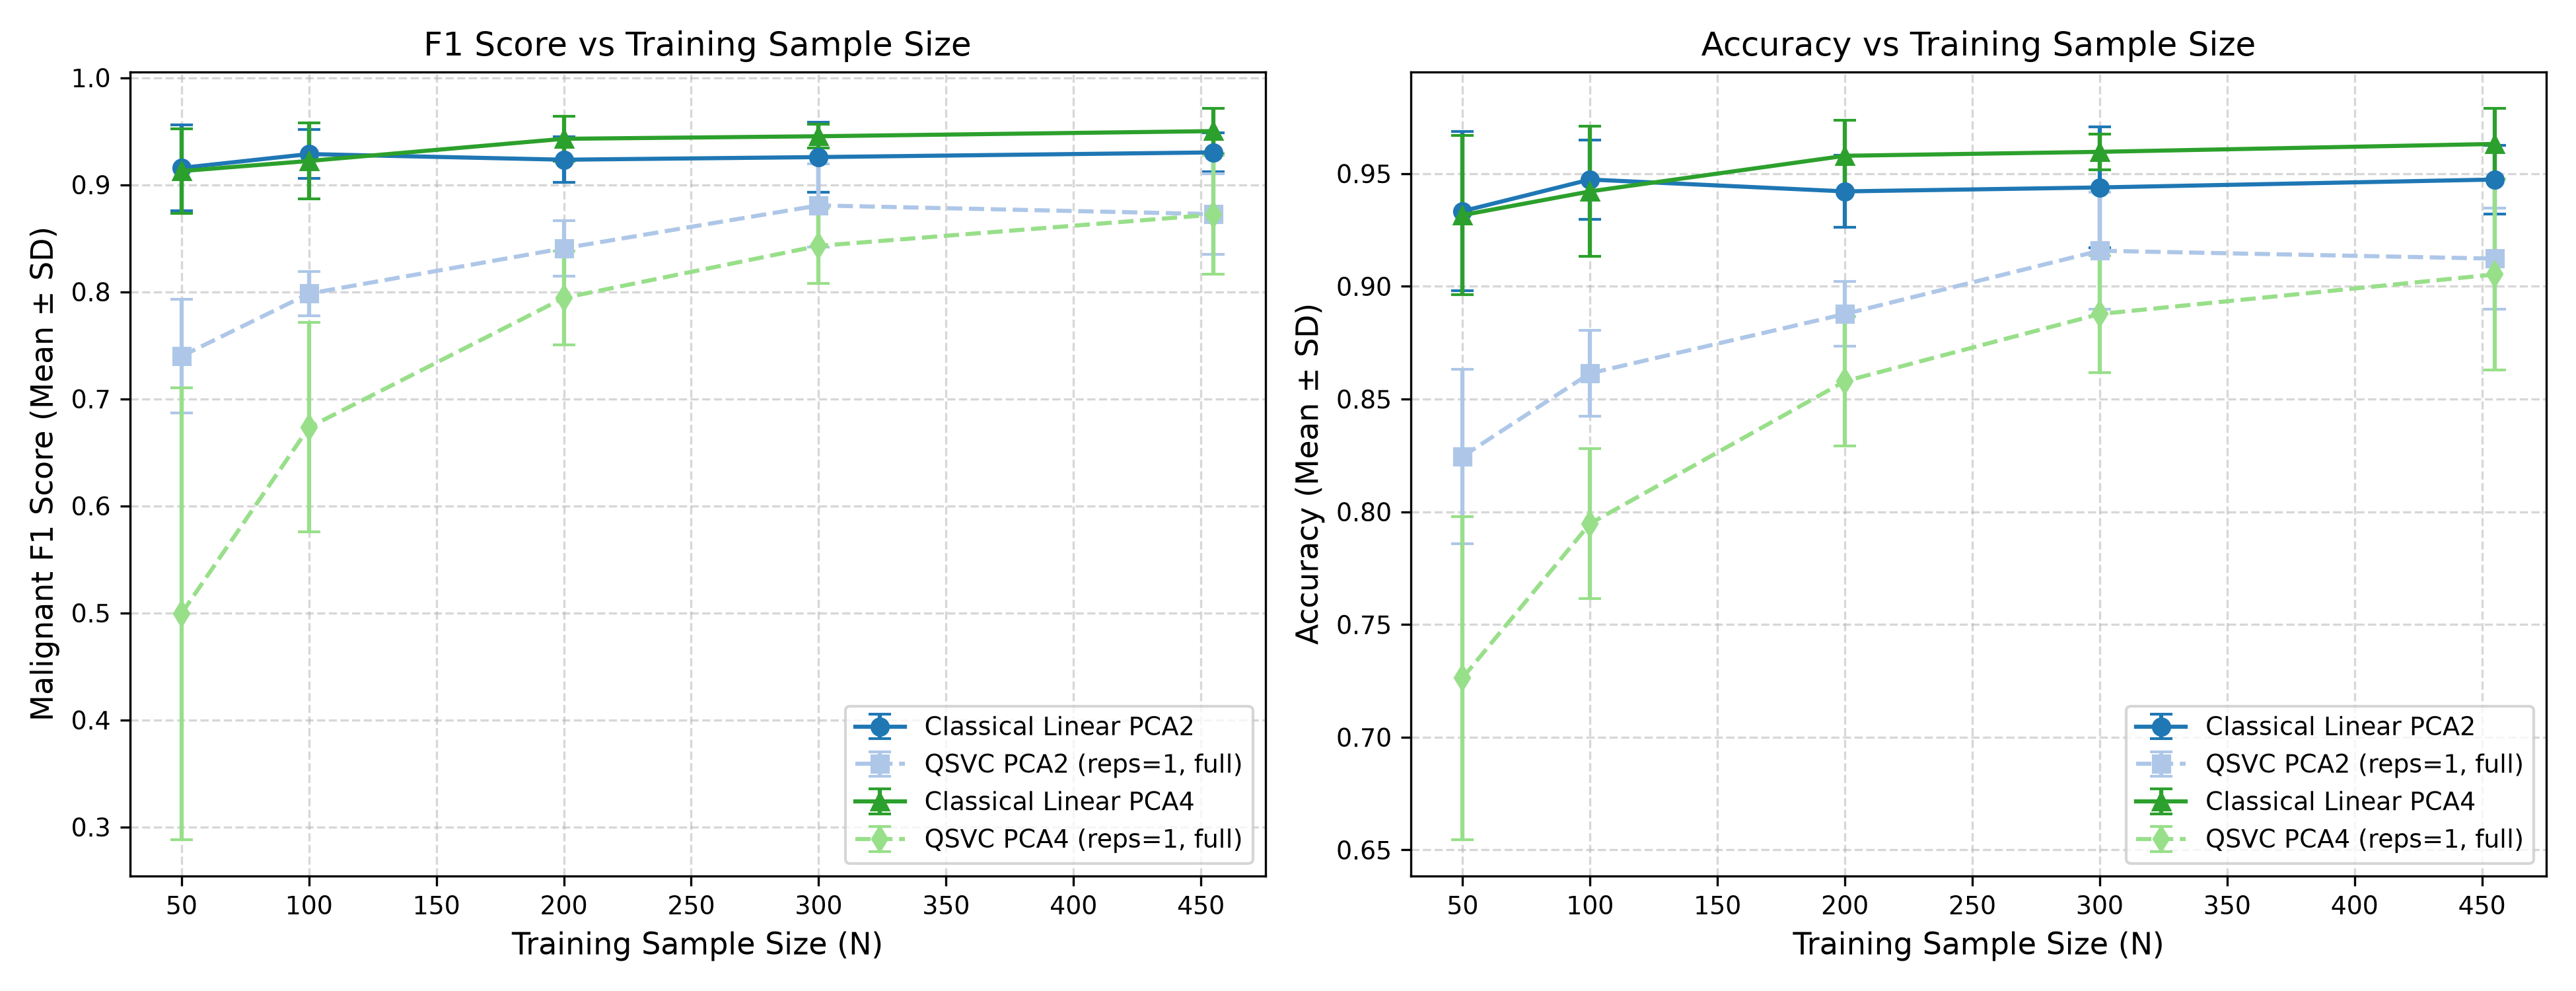
\includegraphics[width=0.95\textwidth]{figures/final_sample_size_scaling.png}
\caption{\textbf{Sample-Size Scaling Dynamics.} Mean malignant F1 score across training subset sizes $N_{\text{train}} \in \{50, 100, 200, 300, 455\}$. Classical SVMs maintain a consistent performance advantage across all sample regimes, with QSVC exhibiting its largest deficit at $N=50$.}
\label{fig:scaling}
\end{figure}

\subsection{Empirical Observations}
\begin{itemize}
    \item \textbf{Absence of Small-Data Quantum Advantage:} At $N_{\text{train}} = 50$, the fixed-hyperparameter classical models retained higher predictive performance:
    \begin{itemize}
        \item Classical Linear SVM (PCA 2): $\text{F1} = 0.9157 \pm 0.0402$, $\text{Accuracy} = 0.9333 \pm 0.0354$
        \item Classical Linear SVM (PCA 4): $\text{F1} = 0.9128 \pm 0.0395$, $\text{Accuracy} = 0.9316 \pm 0.0353$
        \item QSVC (2Q): $\text{F1} = 0.7398 \pm 0.0531$ (performance deficit: $-0.1759$)
        \item QSVC (4Q): $\text{F1} = 0.4994 \pm 0.2110$ (performance deficit: $-0.4134$, with recall collapsing to $0.4095$)
    \end{itemize}
    \item \textbf{Sample Efficiency Convergence:} As training size expanded from $N=50$ to $N=455$, QSVC performance steadily improved (2Q: $0.740 \to 0.873$; 4Q: $0.499 \to 0.872$). However, classical SVMs maintained a substantial lead at every evaluated sample size. Full tabular scaling values are documented in Supplementary Table~S1.
\end{itemize}

\section{Authoritative Nested Predictive Results}
Final authoritative performance metrics from \texttt{results/corrected\_nested/} across the five outer test splits are summarized in Table~\ref{tab:main_perf} and visualized in Figure~\ref{fig:f1_comp}.

\begin{figure}[htbp]
\centering
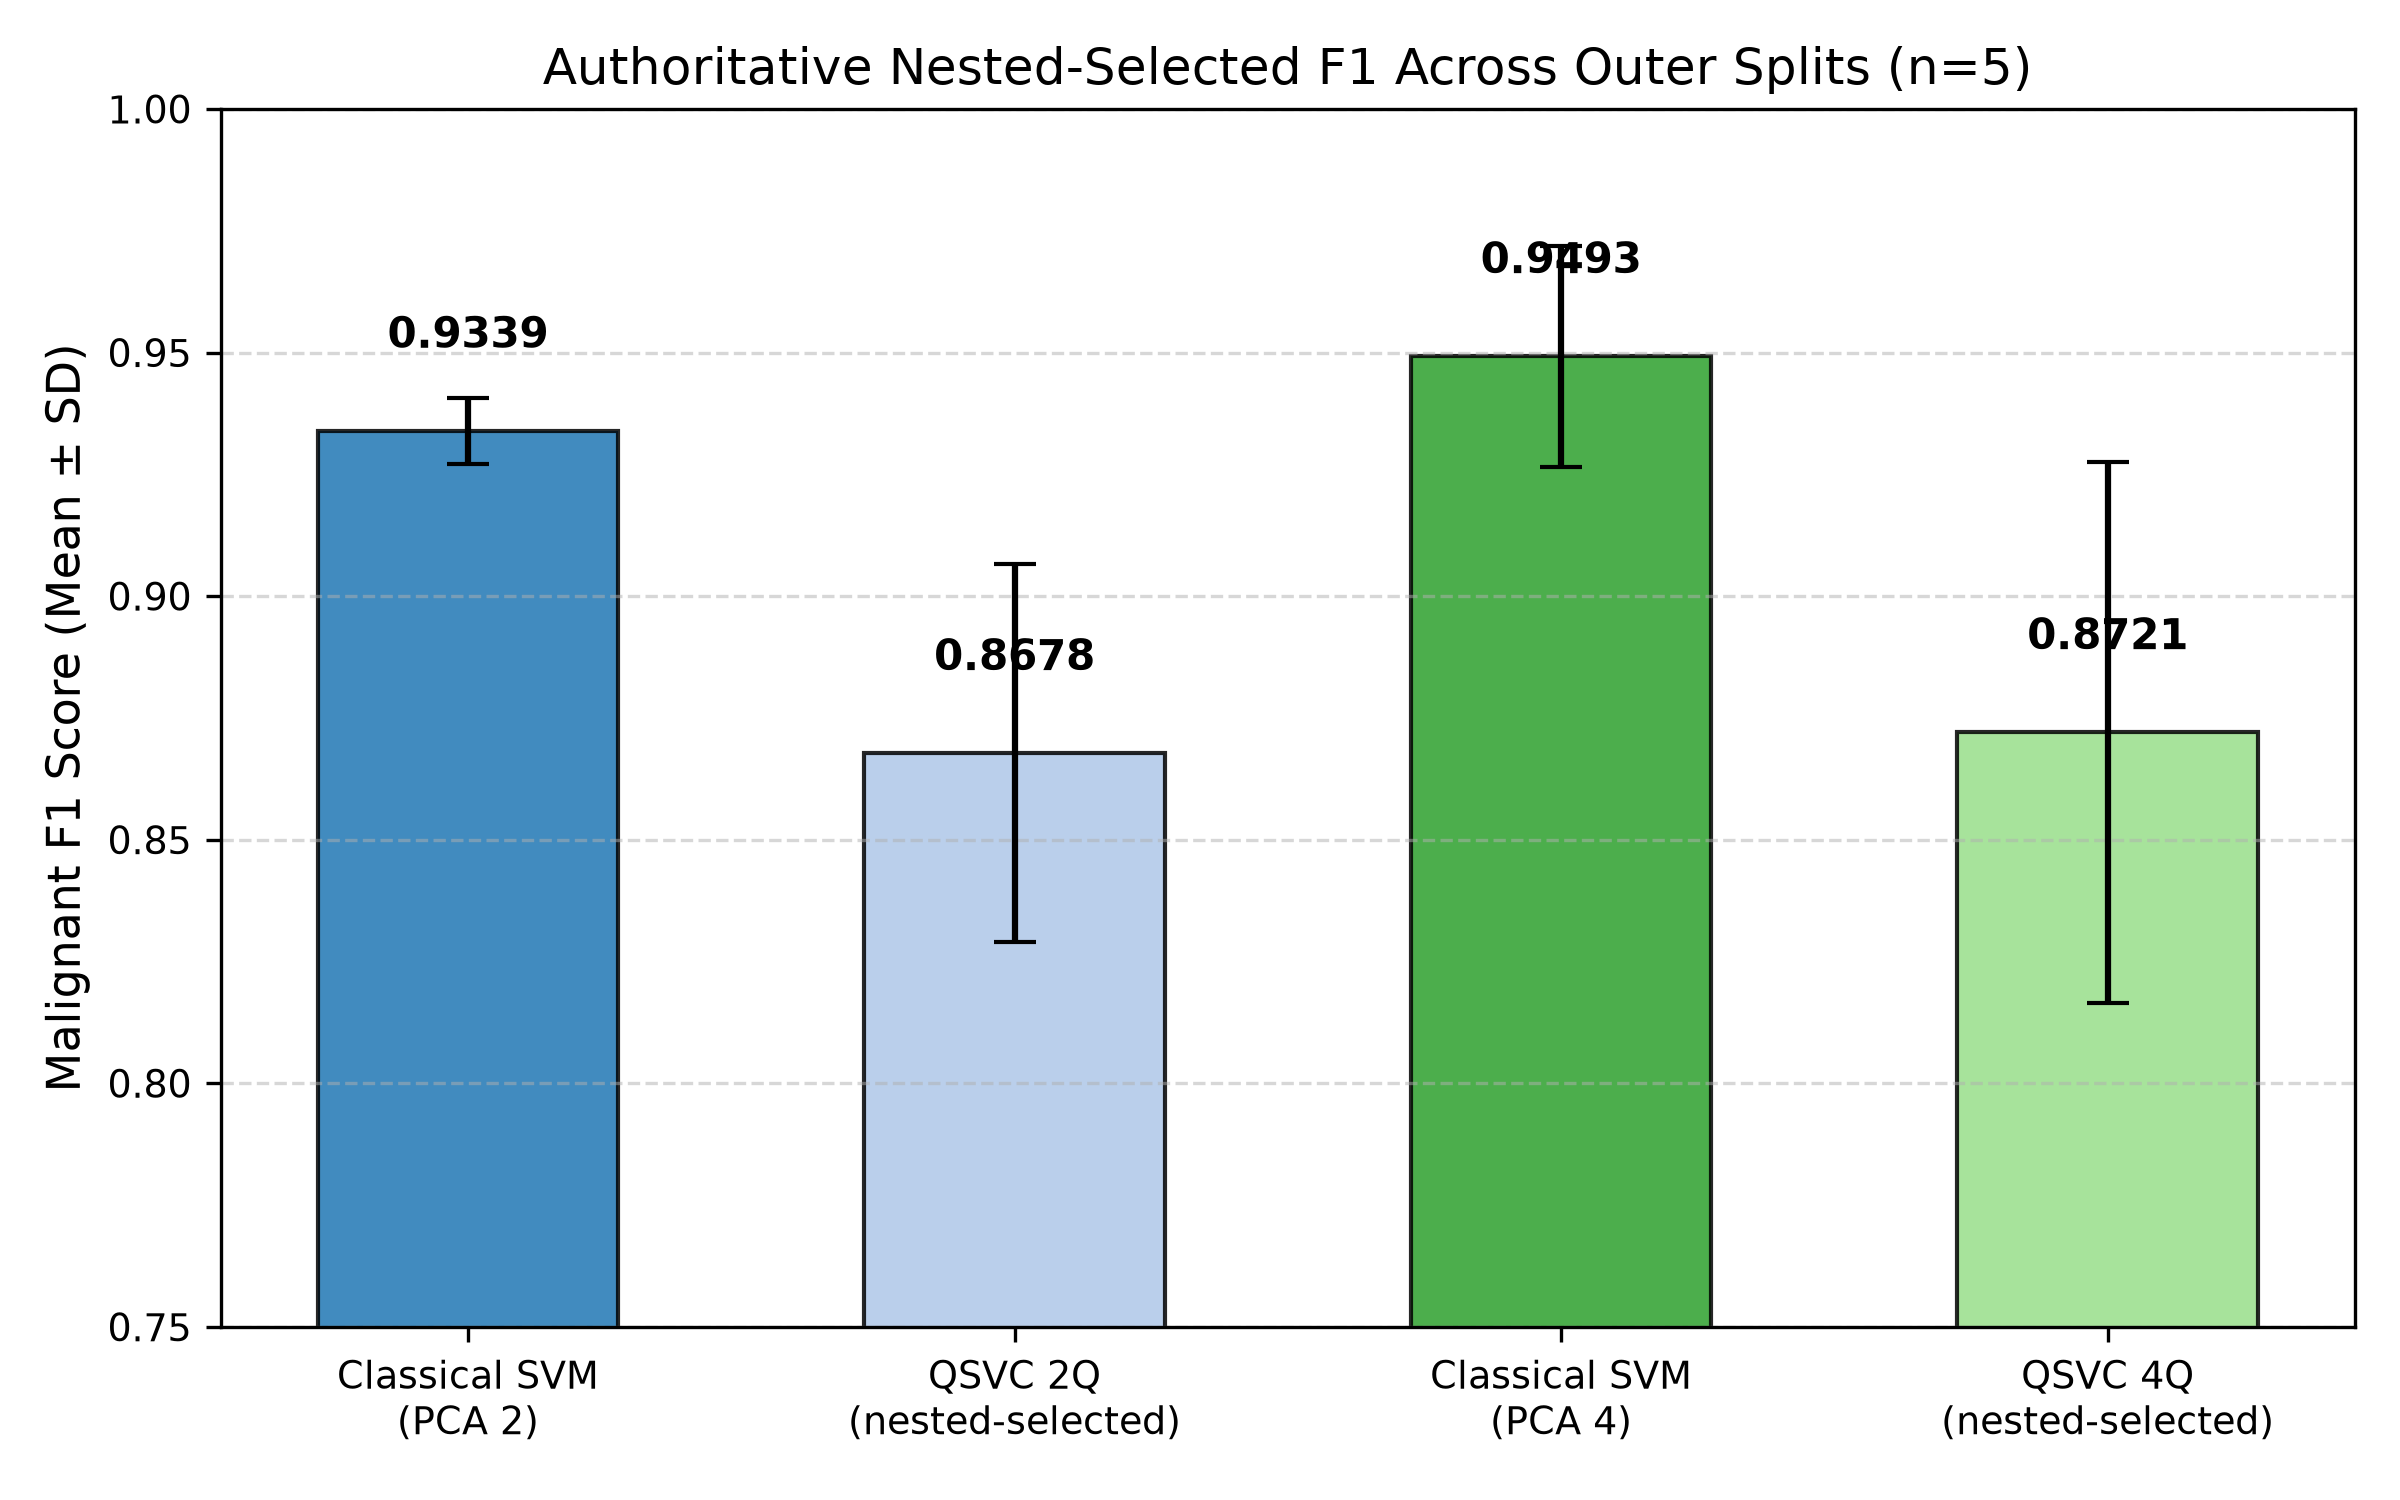
\includegraphics[width=0.85\textwidth]{figures/final_f1_comparison.png}
\caption{\textbf{Final Malignant F1 Score Comparison.} Mean outer-test malignant F1 with sample-standard-deviation error bars for the inner-selected classical comparator and nested-selected QSVC across two- and four-dimensional representations. The classical comparator had higher F1 on 5/5 matched splits in both representations.}
\label{fig:f1_comp}
\end{figure}

\begin{table}[htbp]
\centering
\caption{Authoritative Nested Outer-Test Performance Summary across 5 Outer Splits (Mean $\pm$ SD).}
\label{tab:main_perf}
\vspace{2mm}
\resizebox{\textwidth}{!}{%
\begin{tabular}{llcccccc}
\toprule
Model Architecture & Repr. & Qubits & Test Accuracy & Test Precision & Test Recall & Malignant F1 & Test ROC-AUC \\
\midrule
\textbf{Classical Comparator} & \textbf{PCA 2} & \textbf{0} & $\mathbf{0.9509 \pm 0.0048}$ & $\mathbf{0.9257 \pm 0.0172}$ & $\mathbf{0.9429 \pm 0.0213}$ & $\mathbf{0.9339 \pm 0.0068}$ & $\mathbf{0.9866 \pm 0.0074}$ \\
Tuned Linear SVM & PCA 2 & 0 & $0.9509 \pm 0.0078$ & $0.9266 \pm 0.0318$ & $0.9429 \pm 0.0213$ & $0.9341 \pm 0.0093$ & $0.9894 \pm 0.0030$ \\
Tuned RBF SVM & PCA 2 & 0 & $0.9456 \pm 0.0096$ & $0.9245 \pm 0.0182$ & $0.9286 \pm 0.0238$ & $0.9263 \pm 0.0133$ & $0.9810 \pm 0.0119$ \\
\textbf{Nested-selected QSVC} & \textbf{PCA 2} & \textbf{2} & $\mathbf{0.9070 \pm 0.0237}$ & $\mathbf{0.9064 \pm 0.0457}$ & $\mathbf{0.8381 \pm 0.0832}$ & $\mathbf{0.8678 \pm 0.0388}$ & $\mathbf{0.9644 \pm 0.0244}$ \\
\midrule
\textbf{Classical Comparator} & \textbf{PCA 4} & \textbf{0} & $\mathbf{0.9632 \pm 0.0157}$ & $\mathbf{0.9570 \pm 0.0184}$ & $\mathbf{0.9429 \pm 0.0464}$ & $\mathbf{0.9493 \pm 0.0227}$ & $\mathbf{0.9941 \pm 0.0039}$ \\
Tuned Linear SVM & PCA 4 & 0 & $0.9684 \pm 0.0100$ & $0.9671 \pm 0.0255$ & $0.9476 \pm 0.0391$ & $0.9565 \pm 0.0143$ & $0.9952 \pm 0.0029$ \\
Tuned RBF SVM & PCA 4 & 0 & $0.9561 \pm 0.0139$ & $0.9434 \pm 0.0244$ & $0.9381 \pm 0.0398$ & $0.9401 \pm 0.0198$ & $0.9935 \pm 0.0045$ \\
\textbf{Nested-selected QSVC} & \textbf{PCA 4} & \textbf{4} & $\mathbf{0.9053 \pm 0.0423}$ & $\mathbf{0.8748 \pm 0.0767}$ & $\mathbf{0.8762 \pm 0.0832}$ & $\mathbf{0.8721 \pm 0.0556}$ & $\mathbf{0.9581 \pm 0.0227}$ \\
\bottomrule
\end{tabular}%
}
\end{table}

\subsection{Performance Synthesis}
\begin{enumerate}
    \item \textbf{Primary Endpoint (Malignant F1):} In the 2-dimensional representation, the Classical Comparator achieved a Malignant F1 of $0.9339 \pm 0.0068$, outperforming QSVC 2Q ($0.8678 \pm 0.0388$). In the 4-dimensional representation, the Classical Comparator achieved an F1 of $0.9493 \pm 0.0227$ (with Linear SVM reaching $0.9565 \pm 0.0143$), while QSVC 4Q attained $0.8721 \pm 0.0556$.
    \item \textbf{Secondary Descriptive Endpoints:} Across all secondary metrics (Test Accuracy, Precision, Recall, and ROC-AUC), classical models demonstrated higher descriptive performance. In PCA 2, classical accuracy reached $0.9509 \pm 0.0048$ vs.\ $0.9070 \pm 0.0237$ for QSVC 2Q, with classical recall showing higher sensitivity for malignancy ($0.9429$ vs.\ $0.8381$). In PCA 4, classical accuracy reached $0.9632 \pm 0.0157$ vs.\ $0.9053 \pm 0.0423$ for QSVC 4Q. Classical ROC-AUC exceeded $0.986$ (PCA 2) and $0.994$ (PCA 4), whereas QSVC reached $0.9644$ (2Q) and $0.9581$ (4Q). Under the predefined statistical protocol, these secondary metrics are descriptive and were not subjected to formal hypothesis testing.
\end{enumerate}

\section{Kernel Geometry Analysis}
To analyze the mathematical properties of the feature spaces, we examined the training Gram matrices ($455 \times 455$) using spectral decomposition~\cite{canatar2021spectral, kubler2021inductive}:
\begin{equation}
\text{Effective Rank} = \exp\left( -\sum_{i=1}^N p_i \ln p_i \right), \quad p_i = \frac{\lambda_i}{\sum_j \lambda_j}
\end{equation}
where $\lambda_i$ denote the non-negative eigenvalues of the normalized Gram matrix.

\subsection{Geometry Properties}
\begin{itemize}
    \item \textbf{Two-Qubit Quantum Kernel:} Mean off-diagonal similarity: $0.3244 \pm 0.0071$; off-diagonal std: $0.2908 \pm 0.0039$; effective rank: $7.35 \pm 0.21$.
    \item \textbf{Four-Qubit Quantum Kernel:} Mean off-diagonal similarity: $0.0961 \pm 0.0032$; off-diagonal std: $0.1015 \pm 0.0046$; effective rank: $96.49 \pm 5.41$.
\end{itemize}

\subsection{Mathematical Interpretation and Operator Dimensionality}
A vital theoretical distinction must be maintained between the statevector Hilbert dimension $2^n$ (4 for 2Q, 16 for 4Q) and the linear operator feature space $\mathcal{B}(\mathcal{H})$ whose dimension scales up to $4^n$ (16 for 2Q, 256 for 4Q)~\cite{schuld2019quantum, schuld2021supervised}. Because the fidelity kernel evaluates the Hilbert-Schmidt inner product of density operators $K(\mathbf{x}_i, \mathbf{x}_j) = \text{Tr}[\rho(\mathbf{x}_i)\rho(\mathbf{x}_j)]$, the linear capacity of the kernel Gram matrix is bounded by $4^n$ rather than $2^n$.

For the 2-qubit kernel, mean off-diagonal fidelity was $0.3244 \pm 0.0071$ and effective rank was $7.35 \pm 0.21$; for the 4-qubit kernel, the corresponding values were $0.0961 \pm 0.0032$ and $96.49 \pm 5.41$. Effective rank summarizes the entropy and evenness of the empirical Gram spectrum; it is not a count of occupied physical states. The lower off-diagonal similarities and broader spectrum in 4Q are concentration-like geometric behavior, but two qubit counts cannot establish an asymptotic concentration law or a causal explanation for predictive performance~\cite{thanasilp2024exponential}.

\section{Classical RBF vs.\ Quantum Kernel Alignment}
To quantify similarity between the quantum and classical kernel geometries, we computed \textbf{centered kernel alignment (CKA)} between the quantum Gram matrix $\mathbf{K}$ and the seed-specific tuned classical RBF reference matrix $\mathbf{L}$~\cite{cortes2012centered}:
\begin{equation}
\text{CKA}(\mathbf{K}, \mathbf{L}) = \frac{\langle \mathbf{K}_c, \mathbf{L}_c \rangle_F}{\|\mathbf{K}_c\|_F \|\mathbf{L}_c\|_F}, \quad \mathbf{K}_c = \mathbf{H}\mathbf{K}\mathbf{H}
\end{equation}
where $\mathbf{H} = \mathbf{I} - \frac{1}{N}\mathbf{1}\mathbf{1}^T$ is the empirical centering matrix.

\begin{figure}[htbp]
\centering
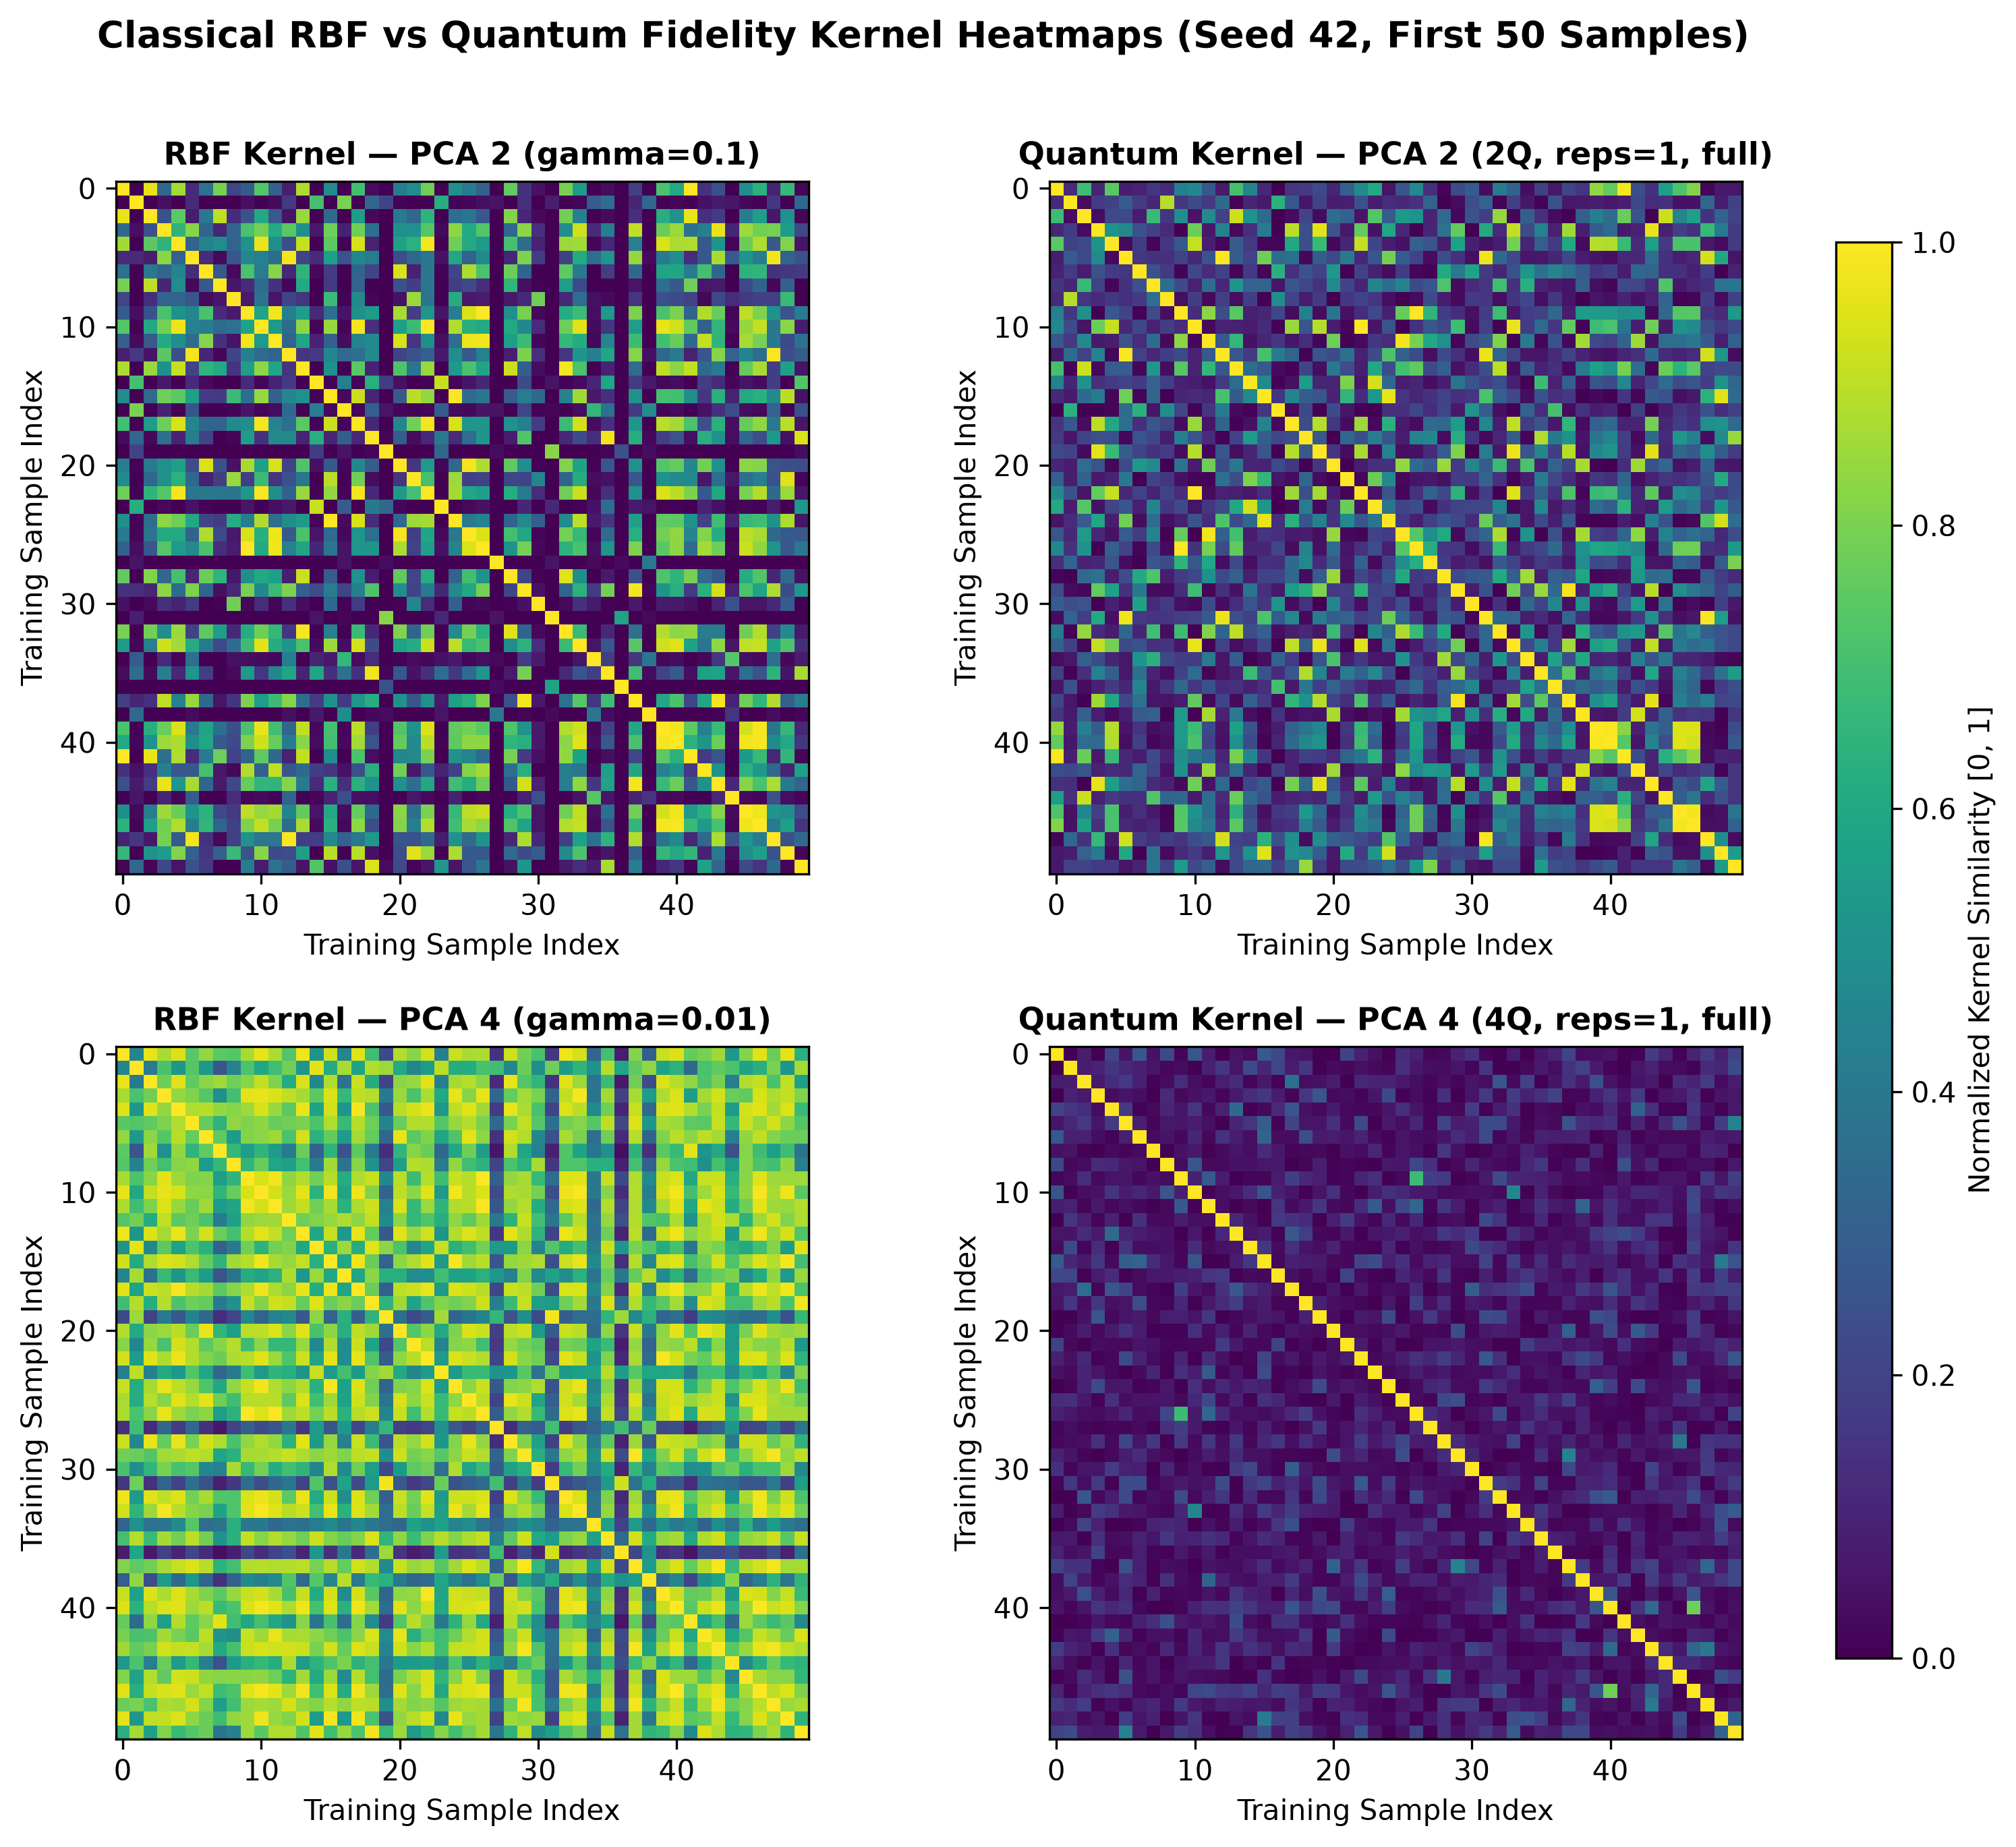
\includegraphics[width=0.95\textwidth]{figures/final_kernel_heatmaps.png}
\caption{\textbf{Classical RBF vs.\ Quantum Kernel Heatmaps.} The first 50 training samples from outer seed 42 are shown for the seed-specific tuned RBF and nested-selected quantum kernels at each representation. CKA summaries use the complete 455-sample training matrices across all five outer splits; the image is illustrative rather than the object of the aggregate calculation.}
\label{fig:heatmaps}
\end{figure}

\begin{table}[htbp]
\centering
\caption{Kernel Geometry and Centered Kernel Alignment (CKA) across 5 Outer Splits (Mean $\pm$ SD).}
\label{tab:cka}
\vspace{2mm}
\resizebox{\textwidth}{!}{%
\begin{tabular}{lcccccc}
\toprule
Repr. / Qubits & CKA Alignment & Uncentered Frob.\ Align. & Class.\ RBF Eff.\ Rank & Quantum Eff.\ Rank & Class.\ RBF Off-Diag & Quantum Off-Diag \\
\midrule
\textbf{PCA 2 / 2Q} & $\mathbf{0.5732 \pm 0.1548}$ & $\mathbf{0.8344 \pm 0.0320}$ & $6.52 \pm 4.15$ & $\mathbf{7.35 \pm 0.21}$ & $0.4895 \pm 0.2362$ & $\mathbf{0.3244 \pm 0.0071}$ \\
\textbf{PCA 4 / 4Q} & $\mathbf{0.3375 \pm 0.0704}$ & $\mathbf{0.7162 \pm 0.0117}$ & $6.97 \pm 5.01$ & $\mathbf{96.49 \pm 5.41}$ & $0.5465 \pm 0.1892$ & $\mathbf{0.0961 \pm 0.0032}$ \\
\bottomrule
\end{tabular}%
}
\end{table}

\subsection{Alignment Results and Scientific Rationale}
\begin{itemize}
    \item \textbf{PCA 2 / 2Q:} Mean CKA $= \mathbf{0.5732 \pm 0.1548}$ (uncentered Frobenius alignment $= 0.8344 \pm 0.0320$).
    \item \textbf{PCA 4 / 4Q:} Mean CKA $= \mathbf{0.3375 \pm 0.0704}$ (uncentered Frobenius alignment $= 0.7162 \pm 0.0117$).
\end{itemize}
The lower mean CKA in 4Q indicates greater geometric divergence from the tuned classical RBF kernels than in 2Q; it does not identify a better representation. In this experiment, the more divergent 4Q geometry did not translate into improved predictive performance. CKA is a descriptive similarity measure, and no threshold was used to classify kernels as equivalent or fundamentally different.

\section{Computational Execution Cost and Complexity}
A comprehensive comparison requires evaluating computational complexity and wall-clock execution cost~\cite{chang2011libsvm, preskill2018quantum}. We report benchmarks measured on standard x86\_64 architecture ($N_{\text{train}}=455, N_{\text{test}}=114$).

\begin{figure}[htbp]
\centering
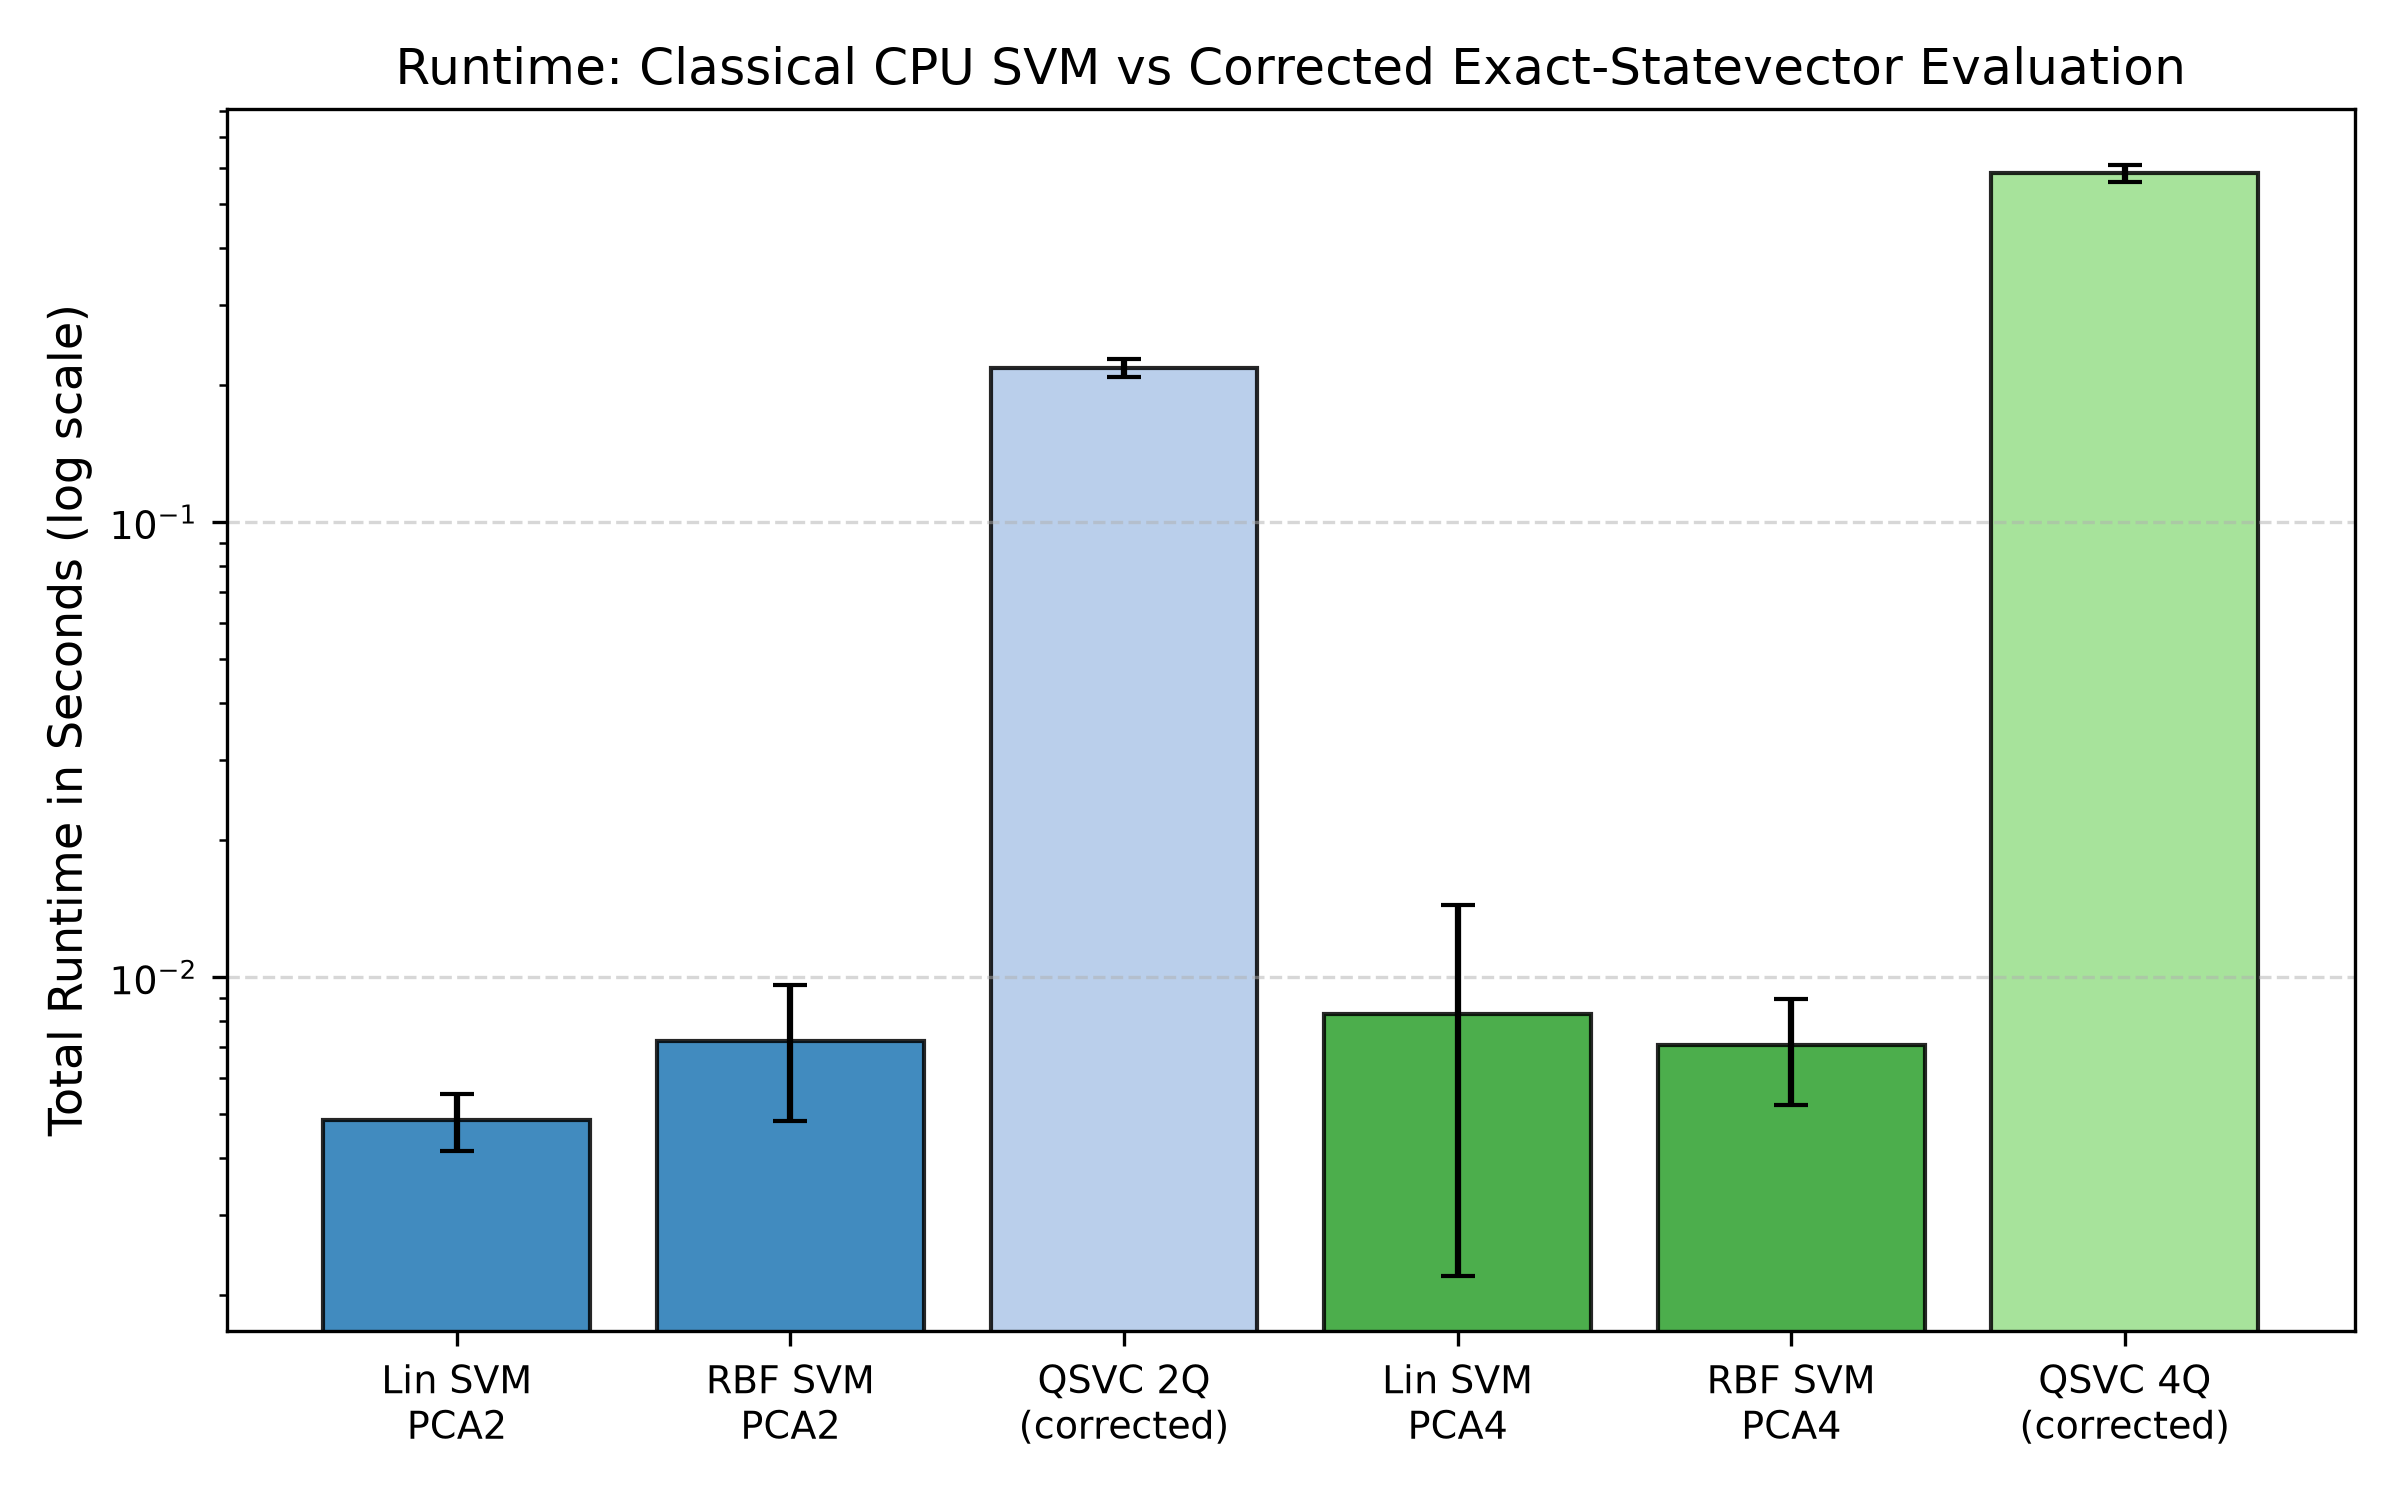
\includegraphics[width=0.85\textwidth]{figures/final_runtime_scaling.png}
\caption{\textbf{Runtime Scaling Comparison.} Wall-clock execution time (seconds) per outer split across classical linear, classical RBF, QSVC 2Q, and QSVC 4Q on classical x86\_64 hardware.}
\label{fig:runtime}
\end{figure}

\subsection{Computational Observations}
\begin{enumerate}
    \item \textbf{Measured Runtime Scope:} The reported \texttt{total\_runtime} includes preprocessing, classifier fitting, and prediction; for QSVC it additionally includes exact statevector generation and train/test Gram products. Inner-search time and kernel-diagnostic time are excluded.
    \item \textbf{Statevector Simulation Overhead:} In the corrected nested outer evaluations, vectorized exact statevector simulation required $0.2181 \pm 0.0096$ seconds for 2Q and $0.5846 \pm 0.0257$ seconds for 4Q on standard x86\_64 architecture---approximately $45\times$ and $71\times$ the corresponding linear-SVM timings.
    \item \textbf{Complexity Separation and Scaling Caveat:} LibSVM SVC training is data-, solver-, and cache-dependent. For this vectorized exact implementation, the dominant dense Gram products have operation count $\mathcal{O}((N_{\text{train}}^2+N_{\text{test}}N_{\text{train}})2^q)$, followed by precomputed-kernel SVC. The measured $\sim 2.7\times$ increase from 2Q to 4Q is an implementation-specific observation from two points, not evidence of an asymptotic law. The measured 2,071,160-byte storage is the combined float64 training and test kernel arrays, not the training Gram matrix alone.
    \item \textbf{Simulation and Hardware:} Statevector timing is not QPU timing~\cite{aaronson2015read}. Physical execution would add compilation, queueing, repeated measurement, noise, and mitigation costs whose values depend on the device and accuracy target. The historical \texttt{ComputeUncompute} timings are measurements from a local pairwise simulator and are reported separately; they are neither physical-hardware timings nor evidence about a fixed shot budget. Complete profiling is provided in Supplementary Table~S2.
\end{enumerate}

\section{Paired Inferential Statistical Analysis}
Paired statistics for the primary endpoint (\textbf{malignant-class F1}) were recomputed from the corrected nested outer-test results across the five matching seeds. The classical-minus-QSVC differences had mean, median, sample SD, and range of $+0.066169$, $+0.069767$, $0.039204$, and $[+0.023529,+0.125387]$ for PCA 2; the corresponding values were $+0.077191$, $+0.088580$, $0.041672$, and $[+0.024363,+0.123701]$ for PCA 4.

\begin{table}[htbp]
\centering
\caption{Paired Statistical Hypothesis Testing on Primary Endpoint (Malignant F1 Score, $n=5$ Splits).}
\label{tab:paired_stat}
\vspace{2mm}
\resizebox{\textwidth}{!}{%
\begin{tabular}{lccccccc}
\toprule
Comparison & Mean Diff ($\bar{\Delta}$) & Median Diff & Wins / Losses / Ties & Wilcoxon $W$ & Exact $p$ & Holm $p$ & Bootstrap 95\% CI \\
\midrule
\textbf{Classical PCA2 vs QSVC PCA2} & $\mathbf{+0.0662}$ & $+0.0698$ & $\mathbf{5 / 0 / 0}$ & 0.0 & 0.0625 & 0.1875 & $\mathbf{[+0.0388, +0.0977]}$ \\
\textbf{Classical PCA4 vs QSVC PCA4} & $\mathbf{+0.0772}$ & $+0.0886$ & $\mathbf{5 / 0 / 0}$ & 0.0 & 0.0625 & 0.1875 & $\mathbf{[+0.0445, +0.1092]}$ \\
\textbf{QSVC PCA2 vs QSVC PCA4} & $\mathbf{-0.0043}$ & $-0.0154$ & $2 / 3 / 0$ & 6.0 & 0.8125 & 0.8125 & $[-0.0291, +0.0201]$ \\
\bottomrule
\end{tabular}%
}
\end{table}

\subsection{Inferential Limitations and Statistical Framing}
\begin{enumerate}
    \item \textbf{Directional Stability:} Across all five evaluated outer seeds, the Classical Comparator achieved higher malignant F1 scores than QSVC without a single exception (5/5 wins for both PCA 2 and PCA 4).
    \item \textbf{Exploratory Bootstrap Intervals:} Non-parametric bootstrap percentile intervals (10,000 resamples over the five observed split differences) fall strictly above zero: $[+0.0388, +0.0977]$ for PCA 2 and $[+0.0445, +0.1092]$ for PCA 4. We explicitly qualify these intervals as exploratory diagnostics over five dependent split-level observations, rather than confirmatory bounds over independent sample cohorts.
    \item \textbf{Small-Sample Power Bound:} Because $n=5$, the minimum achievable two-sided exact Wilcoxon $p$-value when all differences share the same sign is $2 \times (1/2)^5 = 0.0625$ (which adjusts to $0.1875$ under Holm-Bonferroni correction). Therefore, these tests cannot reject the null hypothesis at the conventional $\alpha = 0.05$ significance threshold.
    \item \textbf{Sample Overlap Dependence:} The five outer 80/20 train/test splits reuse observations. Pairwise training-set intersections contain 358--367 samples (mean 362.2), about 79.6\% of each 455-sample training set; pairwise test intersections contain 17--26 samples. The split-level outcomes are therefore not independent experimental replicates, so the Wilcoxon and bootstrap calculations are exploratory.
    \item \textbf{Framing:} Consequently, we refrain from claiming ``statistically significant classical superiority'' in a formal asymptotic sense. We report these findings as highly consistent descriptive evidence of classical advantage under the evaluated experimental constraints.
\end{enumerate}

\section{Discussion}

\subsection{Classical Performance on WDBC}
The WDBC variables are continuous morphometric descriptors derived from digitized cell nuclei~\cite{street1993nuclear}. Strong performance from both linear and RBF SVMs after two- or four-component PCA is consistent with decision structure that these classical kernels can represent effectively. The experiment did not directly identify the data-generating geometry, however, so it cannot establish that either classical kernel is optimal or attribute the performance gap to a single mechanism.

\subsection{Sensitivity of the Quantum Feature Map}
QSVC performance varied substantially across the tested feature maps. In four qubits with full entanglement, increasing \texttt{reps} from 1 to 3 was observed alongside a decrease in malignant F1 from $0.872$ to $0.540$, lower off-diagonal similarity variation, and higher effective rank. This joint pattern is consistent with concentration-like geometry discussed in the literature~\cite{thanasilp2024exponential}, but the ablation does not establish depth as the sole cause or demonstrate asymptotic concentration.

\subsection{Geometric Novelty vs.\ Utility}
Centered kernel alignment was lower for the four-qubit comparison ($\text{CKA} = 0.3375 \pm 0.0704$) than for the two-qubit comparison ($0.5732 \pm 0.1548$). Yet the 4Q QSVC did not improve predictive performance. Lower alignment indicates greater geometric divergence from the selected RBF kernels, not a better quantum representation; task-relevant alignment, rather than distinctness alone, is what matters for prediction~\cite{huang2021power, kubler2021inductive}.

\subsection{Sample Efficiency Findings}
No small-data advantage was observed for QSVC in this experimental setting. At $N_{\text{train}}=50$, 4Q QSVC achieved F1 $\approx 0.499$ and malignant recall $0.4095$, whereas the two fixed-$C$ linear SVM curves remained above $0.91$ F1. This result is specific to the tested subsets and models. It illustrates why theoretical generalization bounds, which concern learnability under stated complexity assumptions, should not be interpreted as guarantees of comparative advantage on classical tabular data~\cite{caro2022generalization}.

\subsection{Computational Trade-Offs}
In the measured CPU implementation, exact statevector QSVC pipelines took roughly 47--80 times as long as the corresponding linear-SVM reference pipelines. This comparison concerns a small exact simulator and includes kernel construction; it does not estimate QPU runtime. Physical devices would introduce different costs and errors, so no hardware speed conclusion follows~\cite{preskill2018quantum, aaronson2015read}.

\subsection{Scope and Boundaries of Conclusions}
To avoid over-generalizing our negative result, we explicitly delineate the scientific scope of our findings:
\begin{itemize}
    \item \textbf{What Was Not Observed:} Within the evaluated Wisconsin Diagnostic Breast Cancer setting---PCA compression to 2 and 4 dimensions, corresponding 2Q and 4Q fixed Second-Order Pauli-Z feature maps, the predefined outer splits, and exact statevector simulation---no QSVC advantage over the tuned classical Linear or RBF SVM comparators was observed in the reported predictive or computational measures.
    \item \textbf{What Remains Open:} These findings do not rule out quantum advantages for: (a) alternative quantum feature maps, including data re-uploading or trainable kernels; (b) projected quantum kernels designed to mitigate concentration~\cite{huang2021power}; (c) larger representations whose simulation cost depends on circuit structure, algorithms, and hardware; or (d) inherently quantum data for which classical kernels may lack a natural representation.
\end{itemize}

\section{Threats to Validity and Study Limitations}
To maintain scientific rigor, we explicitly enumerate the methodological limitations of this study:
\begin{enumerate}
    \item \textbf{Single Tabular Dataset:} The benchmark is evaluated solely on the WDBC dataset ($N=569$). Findings cannot be generalized to image, sequence, graph, or inherently quantum data~\cite{cerezo2022challenges}.
    \item \textbf{Dimensionality Compression:} Input features were compressed via PCA to 2 and 4 dimensions to accommodate NISQ simulation scale, discarding $36.5\%$ and $20.6\%$ of feature variance, respectively.
    \item \textbf{Restricted Qubit Scale:} Evaluation was limited to 2 and 4 qubits. No empirical scaling conclusion can be drawn for larger circuits, whose simulability depends on circuit structure, numerical method, available memory, and hardware~\cite{preskill2018quantum}.
    \item \textbf{Single Feature-Map Family:} Only the standard Second-Order Pauli-Z Expansion (\texttt{ZZFeatureMap}) was evaluated. Alternative quantum embeddings (e.g., data re-uploading~\cite{perezsalinas2020data}, covariant kernels, or trainable quantum kernels) might yield different results.
    \item \textbf{Study-level adaptivity:} The corrected nested analysis removes direct outer-test involvement from the model-selection algorithm. However, it remains a post hoc reanalysis of a dataset and partition set previously examined during exploratory development and therefore should not be interpreted as independent confirmatory validation.
    \item \textbf{Sample Overlap:} The five outer cross-validation splits share training data, violating sample independence assumptions~\cite{bowles2024better}.
    \item \textbf{Limited Statistical Sample:} An outer sample size of $n=5$ limits statistical power, establishing a mathematical lower bound of $p=0.0625$ on the Wilcoxon signed-rank test.
    \item \textbf{Noiseless Simulation:} Results reflect exact statevector linear algebra for the implemented circuits. Physical hardware noise, gate errors, and measurement uncertainty were not modeled, so their direction and magnitude cannot be inferred from this study.
    \item \textbf{No Physical QPU Execution:} Wall-clock runtimes reflect CPU statevector simulation and do not measure physical quantum hardware execution.
    \item \textbf{Non-Clinical Context:} This study is a methodological machine-learning experiment and does not represent clinical diagnostic validation.
    \item \textbf{No External Validation:} All performance estimates use repeated partitions of one public benchmark; there is no independent cohort or cross-site validation.
    \item \textbf{Runtime Generalizability:} Wall-clock ratios are specific to the recorded software stack, CPU, problem size, and implementation, and should not be extrapolated to QPUs or other simulators.
\end{enumerate}

\section{Conclusion and Future Work}
This study conducted a controlled comparison of classical Support Vector Machines and Quantum Support Vector Classifiers on WDBC, with preprocessing and all final model-selection decisions nested inside each outer-training set. Across the evaluated configurations and aggregate predictive metrics:
\begin{enumerate}
    \item Tuned classical SVM baselines consistently achieved higher descriptive predictive accuracy and malignant F1 scores than QSVC (Classical F1 $\approx 0.934$ vs.\ QSVC $\approx 0.868$ in 2Q; Classical F1 $\approx 0.949$ vs.\ QSVC $\approx 0.872$ in 4Q).
    \item Classical models outperformed QSVC across all five outer cross-validation splits without exception (5/5 wins in both 2D and 4D).
    \item QSVC performance was sensitive to the tested feature-map configurations; deeper 4Q full-entanglement maps were associated with lower F1.
    \item QSVC exhibited no small-data sample efficiency advantage, showing its greatest performance deficit at $N=50$.
    \item The 4-qubit quantum kernel had lower mean CKA with the selected RBF kernels ($0.3375 \pm 0.0704$) than the 2-qubit comparison ($0.5732 \pm 0.1548$), but this greater geometric divergence did not improve predictive performance.
\end{enumerate}
\textbf{Central Conclusion:} Under the evaluated experimental conditions, no quantum advantage was observed.

Future investigations should extend this controlled protocol to independent external biomedical cohorts (e.g., METABRIC, TCGA)~\cite{leither2026benchmarking}, trainable and projected quantum kernels that optimize metric alignment prior to classification~\cite{huang2021power, kubler2021inductive}, physical quantum processor (QPU) evaluations incorporating error mitigation~\cite{preskill2018quantum, peters2021machine}, and non-tabular data structures where quantum feature maps may possess a stronger inductive bias.

\section*{Methodological Correction Note}
During exploratory development, outer-test performance was used to examine feature-map architectures. Before submission, the full QSVC architecture and $C$ search was rerun entirely within nested inner cross-validation. The corrected search independently selected the same effective architectures and seed-specific $C$ values, and final aggregate metrics were unchanged to numerical precision. Historical exploratory artifacts remain preserved for traceability; \texttt{results/corrected\_nested/} is authoritative for final QSVC metrics and paired comparisons.

\section*{Data Availability Statement}
The empirical benchmarking in this study utilizes the publicly available Wisconsin Diagnostic Breast Cancer (WDBC) benchmark dataset originating from the UCI Machine Learning Repository~\cite{street1993nuclear} and distributed via scikit-learn~\cite{pedregosa2011scikit}. The author claims no proprietary rights over the diagnostic data. The \texttt{v1.0.0} release preserves the historical benchmark; corrected authoritative outputs are recorded at repository checkpoint \texttt{f4c8418} and must be included in the next archival release before submission (\url{https://github.com/SinaQP/SVM-Vs-QSVM}).

\section*{Code Availability Statement}
All software implementations are available in the open-source repository \url{https://github.com/SinaQP/SVM-Vs-QSVM}. The historical benchmark is tagged \texttt{v1.0.0}; the corrected nested-selection implementation and outputs are recorded at checkpoint \texttt{f4c8418}. The pipeline is verifiable through the included test suite and validation scripts.

\section*{Author Declarations}
\subsection*{Ethics Approval and Biomedical Statement}
This study used a publicly available benchmark dataset and did not involve the recruitment of human participants or collection of new clinical data.

\subsection*{Author Contributions (CRediT Taxonomy)}
Conceptualization: Sina Qasempour; Methodology: Sina Qasempour; Software: Sina Qasempour; Validation: Sina Qasempour; Formal Analysis: Sina Qasempour; Investigation: Sina Qasempour; Data Curation: Sina Qasempour; Writing -- Original Draft: Sina Qasempour; Writing -- Review \& Editing: Sina Qasempour; Visualization: Sina Qasempour; Project Administration: Sina Qasempour.

\subsection*{Funding Statement}
This research received no external funding.

\subsection*{Conflicts of Interest}
The author declares no conflict of interest.

\subsection*{Acknowledgments}
The author acknowledges the developers and maintainers of Python, scikit-learn, Qiskit, NumPy, SciPy, and matplotlib, whose open-source software made this reproducible benchmark possible.

Generative-AI tools were used during this work for coding and debugging assistance, methodological and statistical review, literature and citation support, scientific writing and editing, visualization workflows, and repository and documentation tasks. The tools were OpenAI Codex (GPT-5.6 Sol) and Google Antigravity (3.8 Flash). Research figures were generated conventionally with Python/Matplotlib from stored numerical artifacts; AI assistance concerned plotting code, workflow, captions, and review rather than direct image synthesis. Reported numerical results were obtained by executing the repository's reproducible computational workflows and checked against stored result artifacts. The author reviewed the generated code, analyses, citations, and manuscript content, made the final scientific decisions, and takes full responsibility for the work. No AI system is credited with authorship.

\bibliographystyle{ieeetr}
\bibliography{references}

\end{document}
